\documentclass[12pt]{exam}

\usepackage{setspace}
\usepackage{listings}
\usepackage{graphicx,subfigure,wrapfig}
\usepackage{multirow}
\usepackage{amsmath}
\usepackage{amssymb}
\usepackage{multicol}
\usepackage{xcolor} 
\usepackage{tikz}
\usepackage{pgfplots}
\usepackage{booktabs}
\usepackage[margin=18mm]{geometry}
\usepackage{xepersian}

\renewcommand{\thepartno}{\harfinumeral{\value{partno}}}
\renewcommand{\partlabel}{(\thepartno)}

\settextfont[
  ExternalLocation=fonts/,
  BoldFont=XB NiloofarBd.ttf,
  ItalicFont=XB NiloofarIt.ttf,
  BoldItalicFont=XB NiloofarBdIt.ttf
]{XB Niloofar.ttf}

\newcommand{\class}{پروژه درس آمار و کاربرد آن}
\newcommand{\term}{نیم‌سال اول \lr{05-06}}
\newcommand{\college}{دانشکده علوم ریاضی}
\newcommand{\prof}{استاد: دکتر علیشاهی}

\singlespacing
\parindent 0ex
\parskip 4pt
\sloppy
\emergencystretch=3em
\renewcommand{\arraystretch}{0.92}

\lstset{
keywordstyle=\textbf,
identifierstyle=, 
stringstyle=\ttfamily,
commentstyle=\color{LimeGreen}, 
numberstyle=\footnotesize,
showstringspaces=false} 
\pgfplotsset{compat=1.18}

\begin{document}

\pagestyle{head}
\firstpageheader{}{}{}
\runningheader{صفحه \thepage\ از \numpages}{}{\class}
\runningheadrule
\begin{tabular}{p{.7\textwidth} l}
\multicolumn{2}{c}{\textbf{به نام خدا}}\\
\multirow{2}{*}{\includegraphics[scale=0.2]{images/logo.png}} & \\ \\
&  \textbf{\class}\\
&  \textbf{\term}\\
&  \textbf{\prof}\\ \\
 \textbf{\college} &  \\
\end{tabular}\\

\rule[1ex]{\textwidth}{.1pt}
\noindent
\textbf{گزارش فاز اول}
\hfill
\textbf{آیدا عامری}
\hfill
\textbf{\lr{403100202}}
\rule[1ex]{\textwidth}{.1pt}


\section{منشأ داده و سازوکار جمع‌آوری}

\subsection{منبع رسمی و دوره زمانی جمع‌آوری داده}
داده‌های این پژوهش از پیمایش ملی بررسی سلامت و تغذیه ایالات متحده آمریکا (\lr{NHANES}) استخراج شده‌اند که توسط مرکز ملی آمار سلامت (\lr{NCHS})، زیرمجموعه مرکز کنترل و پیشگیری از بیماری‌ها (\lr{CDC}) اجرا می‌شود. دوره زمانی مورد بررسی، چرخه اوت \lr{2021} تا اوت \lr{2023} است که فایل‌های آن با پسوند \lr{\_L} نام‌گذاری شده‌اند. این چرخه نخستین انتشار رسمی داده‌های ملی \lr{NHANES} پس از وقفه ناشی از همه‌گیری کووید-\lr{19} محسوب می‌شود. پیش از این، نمونه‌گیری چرخه \lr{2019-2020} در مارس \lr{2020} متوقف شده بود؛ پس از یک وقفه \lr{16} ماهه، عملیات میدانی در اوت \lr{2021} با یک طراحی نمونه بازنگری‌شده از سر گرفته شد تا ضمن حفظ اعتبار آماری، تماس‌های حضوری به حداقل برسد.

\subsection{ماهیت مطالعه و سازوکار تولید داده}
از دیدگاه روش‌شناسی آماری (مطابق فصل اول کتاب ووناکات)، این مجموعه داده حاصل یک پیمایش مقطعی (\lr{Cross-sectional Survey}) و یک مطالعه کاملاً مشاهده‌ای (\lr{Observational Study}) است. برخلاف آزمایش‌های تصادفی کنترل‌شده (\lr{RCT}) که در آن‌ها پژوهشگر مداخله‌ای مانند مصرف سیگار یا ویپ را به صورت تصادفی به افراد تخصیص می‌دهد، در این مطالعه افراد صرفاً بر اساس رفتار طبیعی زندگی خود مشاهده، مصاحبه و آزمایش شده‌اند. بنابراین، روابط آماری استخراج‌شده نشان‌دهنده همبستگی (\lr{Association}) بوده و به تنهایی اثبات‌کننده رابطه علی (\lr{Causal}) مستقیم نیستند. سازوکار تولید داده در این چرخه شامل سه گام متوالی بوده است:
\begin{enumerate}
\item \textbf{غربالگری اولیه خانوار (\lr{Household Screening}):} برای کاهش تماس حضوری در دوره پساکرونا، ابتدا از طریق چهار نوبت ارسال پستی، از خانوارها دعوت شد تا پرسش‌نامه واجد شرایط بودن را به صورت اینترنتی، کاغذی یا تلفنی تکمیل کنند (\lr{Multi-mode screening}) و مراجعه حضوری تنها برای خانوارهای بی‌پاسخ انجام شد.
\item \textbf{مصاحبه جامع سلامت (\lr{Health Interview}):} اطلاعات جمعیت‌شناختی، اقتصادی، تاریخچه مصرف سیگار (\lr{SMQ\_L}) و وضعیت دود داخل منزل (\lr{SMQFAM\_L}) توسط مصاحبه‌گران ثبت گردید.
\item \textbf{معاینات فیزیکی و آزمایشگاهی (\lr{MEC Examination}):} شرکت‌کنندگان به مراکز معاینه سیار (\lr{MEC}) مراجعه کردند. در این مراکز، نمونه‌گیری خون وریدی (\lr{Phlebotomy}) انجام شد و پرسش‌نامه حساس مصرف اخیر دخانیات و ویپ در \lr{5} روز گذشته (\lr{SMQRTU\_L}) هم‌زمان با خون‌گیری تکمیل گردید. نمونه‌های سرم و خون کامل سپس در آزمایشگاه‌های مرجع برای سنجش دقیق متابولیت‌های نیکوتین، فلزات سنگین و شمارش سلول‌های خونی آنالیز شدند.
\end{enumerate}

\subsection{وضعیت دسترسی و محدودیت‌های اخلاقی داده}
داده‌های \lr{NHANES} به دو دسته فایل‌های عمومی (\lr{Public-Use}) و فایل‌های محدود (\lr{RDC Only}) تقسیم می‌شوند. در این پروژه صرفاً از هفت فایل عمومی و بدون محدودیت دسترسی (\lr{Use Constraints: None}) با فرمت استاندارد \lr{SAS Transport (.XPT)} استفاده شده است که میان سپتامبر \lr{2024} تا اوت \lr{2026} منتشر شده‌اند. برای حفظ محرمانگی هویت افراد در این فایل‌های عمومی، شناسه‌های جغرافیایی حذف شده، سن افراد \lr{80} سال و بالاتر با کد سقف \lr{80} (\lr{Top-coded}) و نسبت درآمد به خط فقر بالاتر از \lr{5} با عدد \lr{5.0} ثبت شده است.


\section{واحد مشاهده و ساختار داده}

\subsection{تعریف واحد مشاهده و کلید اتصال}
واحد مشاهده (\lr{Unit of Observation}) و واحد تحلیل در تمامی هفت فایل این پروژه، یک فرد یا شرکت‌کننده انسانی (\lr{Individual Participant}) است که با شماره توالی منحصر‌به‌فرد \lr{SEQN} شناسایی می‌شود. در هر یک از این هفت فایل، هر سطر دقیقاً نماینده یک فرد یکتا است و \lr{SEQN} نقش کلید اصلی (\lr{Primary Key}) و کلید ادغام را ایفا می‌کند. بنابراین میان تمامی فایل‌های مورد استفاده ما یک رابطه یک‌به‌یک (\lr{One-to-One}) در سطح فرد برقرار است (برخلاف فایل‌های غذایی مانند \lr{DR1IFF\_L} که چندسطری هستند و در دامنه این پژوهش قرار ندارند).

\subsection{بررسی ساختارهای تکرارشونده و سلسله‌مراتبی}
این مطالعه طولی (\lr{Longitudinal}) نیست و هر فرد تنها یک بار در چرخه \lr{2021-2023} آزمایش شده است؛ با این حال، در درون یک سطر، متغیرهایی مانند کوتینین (\lr{LBXCOT}) و هیدروکسی‌کوتینین (\lr{LBXHCOT}) از یک نمونه سرم واحد استخراج شده‌اند و از نظر بیولوژیکی وابسته‌اند. از سوی دیگر، نحوه انتخاب افراد دارای ساختار سلسله‌مراتبی و خوشه‌ای چهارمرحله‌ای (شهرستان، بخش، خانوار و فرد) است. افرادی که در یک خوشه جغرافیایی یا خانوار مشترک زندگی می‌کنند، ممکن است از نظر مواجهه‌های محیطی به یکدیگر شبیه‌تر باشند. این ساختار سلسله‌مراتبی در فایل \lr{DEMO\_L} از طریق واحد نمونه‌گیری اولیه ساختگی (\lr{SDMVPSU}) و طبقه ساختگی (\lr{SDMVSTRA}) کدگذاری شده است.

\begin{table}[htbp]
\centering
\caption{ساختار فایل‌های مورد استفاده و ارتباط آن‌ها با واحد مشاهده}
\resizebox{0.92\textwidth}{!}{
\begin{tabular}{lllll}
\toprule
نام فایل & بخش (\lr{Component}) & واحد هر سطر & کلید اتصال & متغیر وزن موجود در فایل \\
\midrule
\lr{DEMO\_L} & جمعیت‌شناختی & یک فرد (\lr{Participant}) & \lr{SEQN} & \lr{WTINT2YR}, \lr{WTMEC2YR} \\
\lr{SMQ\_L} & پرسش‌نامه تاریخچه سیگار & یک فرد (\lr{Participant}) & \lr{SEQN} & ندارد (استفاده از وزن پایه) \\
\lr{SMQRTU\_L} & پرسش‌نامه مصرف \lr{5} روز اخیر & یک فرد (\lr{Participant}) & \lr{SEQN} & ندارد (پرسش در مرکز \lr{MEC}) \\
\lr{SMQFAM\_L} & پرسش‌نامه دود منزل & یک فرد (\lr{Participant}) & \lr{SEQN} & ندارد (استفاده از وزن پایه) \\
\lr{COT\_L} & آزمایشگاه (سرم خون) & یک فرد (\lr{Participant}) & \lr{SEQN} & ندارد (هم‌تراز با خون‌گیری) \\
\lr{PBCD\_L} & آزمایشگاه (خون کامل) & یک فرد (\lr{Participant}) & \lr{SEQN} & \lr{WTPH2YR} \\
\lr{CBC\_L} & آزمایشگاه (خون کامل) & یک فرد (\lr{Participant}) & \lr{SEQN} & \lr{WTPH2YR} \\
\bottomrule
\end{tabular}
}
\end{table}


\section{نمونه‌گیری، انتخاب و قابلیت تعمیم}

\subsection{طراحی نمونه‌گیری احتمالی و تغییرات دوره پساکرونا (\lr{2021-2023})}
انتخاب افراد در \lr{NHANES} یک نمونه‌گیری تصادفی ساده (\lr{SRS}) نیست، بلکه یک نمونه‌گیری احتمالی چهارمرحله‌ای، طبقه‌بندی‌شده و خوشه‌ای است: (۱) انتخاب \lr{30} شهرستان یا واحد اولیه (\lr{PSU})، (۲) انتخاب بخش‌های جغرافیایی (\lr{Segments})، (۳) انتخاب واحدهای مسکونی و خانوارها، و (۴) انتخاب افراد واجد شرایط درون خانوار. بر اساس راهنمای تحلیلی \lr{CDC}، طراحی نمونه در چرخه \lr{2021-2023} دچار دو تغییر بنیادین نسبت به دوره‌های پیشین شده است:
\begin{enumerate}
\item \textbf{حذف بیش‌نمونه‌گیری (\lr{Oversampling}) اقلیت‌های نژادی و کم‌درآمد:} در دوره‌های قبل، برای افزایش دقت برآورد در اقلیت‌ها، بسیاری از خانوارها پس از غربالگری کنار گذاشته می‌شدند (\lr{Walk-aways}). در دوره \lr{2021-2023} برای کاهش مراجعات حضوری، این پیش‌تخصیص حذف شد و در هر خانوار واجد شرایط حداقل یک بزرگسال انتخاب گردید. پیامد آماری این تغییر، افزایش سهم سفیدپوستان غیرهیسپانیک و کاهش حجم نمونه خام اقلیت‌های نژادی است.
\item \textbf{انتخاب کامل سالمندان و کودکان در درون خانوار:} در این چرخه، تمامی اعضای خانوار در بازه سنی \lr{0} تا \lr{19} سال و \lr{60} سال و بالاتر با احتمال \lr{100\%} انتخاب شدند، در حالی که بزرگسالان \lr{20} تا \lr{59} ساله به صورت تصادفی (\lr{1} یا \lr{2} نفر از هر خانوار) انتخاب گردیدند. این امر باعث بیش‌نمایی چشمگیر سالمندان بالای \lr{60} سال در نمونه خام شده است.
\end{enumerate}

\subsection{تورش عدم پاسخ، وزن‌دهی و دامنه تعمیم‌پذیری}
در چرخه \lr{2021-2023}، نرخ پاسخ‌دهی بدون وزن کاهش یافت؛ به طوری که نرخ پاسخ به غربالگری \lr{65.6\%}، مشارکت در مصاحبه \lr{34.6\%} و حضور در مرکز معاینات (\lr{MEC}) \lr{25.7\%} گزارش شد (در مقایسه با \lr{51.0\%} و \lr{46.9\%} در دوره پیشاکرونا). همچنین برخی مراجعه‌کنندگان به کلینیک از دادن نمونه خون وریدی خودداری کردند. برای رفع تورش عدم پاسخ (\lr{Nonresponse Bias}) و جبران شانس نابرابر انتخاب، مرکز \lr{NCHS} برای نخستین بار وزن اختصاصی دو ساله خون‌گیری (\lr{WTPH2YR}) را منتشر کرده است. بدون اعمال این وزن، نتایج صرفاً توصیف‌کننده نمونه خام (با بیش‌نمایی سالمندان و سفیدپوستان) است؛ اما با اعمال وزن \lr{WTPH2YR}، نتایج قابلیت تعمیم معتبر به کل جمعیت بزرگسال غیرنظامی و غیرنهادی ایالات متحده آمریکا (\lr{U.S. civilian noninstitutionalized population}) در بازه اوت \lr{2021} تا اوت \lr{2023} را خواهد داشت.


\section{طبقه‌بندی متغیرها و مقیاس اندازه‌گیری}

انتخاب شاخص‌های خلاصه عددی، نمودارها و مدل‌های استنباطی مستقیماً به مقیاس اندازه‌گیری متغیرها وابسته است. متغیرهای پاسخ شامل غلظت کوتینین سرم (\lr{LBXCOT})، هیدروکسی‌کوتینین (\lr{LBXHCOT})، کادمیوم خون (\lr{LBXBCD})، سرب خون (\lr{LBXBPB})، هموگلوبین (\lr{LBXHGB}) و شمارش گلبول‌های سفید (\lr{LBXWBCSI}) همگی از نوع کمی پیوسته (\lr{Continuous}) و در مقیاس نسبی (\lr{Ratio Scale}) هستند؛ زیرا دارای صفر مطلق و معنادار بوده و امکان اعمال تبدیل لگاریتمی و رگرسیون خطی (\lr{OLS}) را فراهم می‌کنند.

متغیر توضیحی اصلی یعنی «گروه مصرف دخانیات» (\lr{Smoking\_Group}) که از ترکیب منطقی وضعیت فعلی سیگار (\lr{SMQ040})، مصرف سیگار در \lr{5} روز اخیر (\lr{SMQ681}) و مصرف ویپ در \lr{5} روز اخیر (\lr{SMQ846}) ساخته می‌شود، یک متغیر طبقه‌ای اسمی (\lr{Nominal}) چهارسطحی (غیرسیگاری، انحصاری ویپ، انحصاری سیگار و مصرف دوگانه) است که در فاز اول با جدول فراوانی و نمودار جعبه‌ای، در فاز سوم با تحلیل واریانس (\lr{ANOVA}) و در فاز چهارم با متغیرهای مجازی (\lr{Dummy}) تحلیل می‌شود. متغیرهای تعداد روز و تعداد نخ مصرفی (\lr{SMQ710}، \lr{SMQ720} و \lr{SMQ849}) و تعداد سیگاری‌های منزل (\lr{SMD470}) از نوع کمی گسسته (شمارشی) بوده و کدهای کامنت آزمایشگاهی (\lr{LBDCOTLC} و \lr{LBDBCDLC}) متغیرهایی طبقه‌ای و دودویی (\lr{0}: بالای حد تشخیص، \lr{1}: زیر حد تشخیص \lr{LOD}) هستند.

\begin{table}[htbp]
\centering
\caption{طبقه‌بندی، مقیاس اندازه‌گیری و نقش متغیرهای پژوهش}
\resizebox{\textwidth}{!}{
\begin{tabular}{llllll}
\toprule
نام متغیر & فایل مبدأ & شرح متغیر و واحد اندازه‌گیری & نوع متغیر & مقیاس آماری & نقش در تحلیل \\
\midrule
\lr{LBXCOT} & \lr{COT\_L} & غلظت کوتینین سرم (\lr{ng/mL}) & کمی پیوسته & نسبی (\lr{Ratio}) & پاسخ اصلی (\lr{$Y_1$}) \\
\lr{LBXBCD} & \lr{PBCD\_L} & غلظت کادمیوم خون (\lr{ug/L}) & کمی پیوسته & نسبی (\lr{Ratio}) & پاسخ اصلی (\lr{$Y_2$}) \\
\lr{LBXHCOT} & \lr{COT\_L} & هیدروکسی‌کوتینین سرم (\lr{ng/mL}) & کمی پیوسته & نسبی (\lr{Ratio}) & پاسخ مکمل / حساسیت \\
\lr{LBXBPB} & \lr{PBCD\_L} & غلظت سرب خون (\lr{ug/dL}) & کمی پیوسته & نسبی (\lr{Ratio}) & پاسخ مکمل / همبستگی \\
\lr{LBXHGB} & \lr{CBC\_L} & غلظت هموگلوبین خون (\lr{g/dL}) & کمی پیوسته & نسبی (\lr{Ratio}) & پیامد بالینی مکمل \\
\lr{LBXWBCSI} & \lr{CBC\_L} & شمارش گلبول سفید (\lr{1000 cells/uL}) & کمی پیوسته & نسبی (\lr{Ratio}) & پیامد التهابی مکمل \\
\lr{SMQ040} & \lr{SMQ\_L} & وضعیت فعلی کشیدن سیگار & طبقه‌ای & ترتیبی (\lr{Ordinal}) & ساخت گروه مصرف (\lr{$X$}) \\
\lr{SMQ681} & \lr{SMQRTU\_L} & مصرف تنباکوی تدخینی در \lr{5} روز اخیر & طبقه‌ای & دودویی (\lr{Binary}) & ساخت گروه مصرف (\lr{$X$}) \\
\lr{SMQ846} & \lr{SMQRTU\_L} & مصرف سیگار الکترونیکی در \lr{5} روز اخیر & طبقه‌ای & دودویی (\lr{Binary}) & ساخت گروه مصرف (\lr{$X$}) \\
\lr{SMQ710} & \lr{SMQRTU\_L} & تعداد روز مصرف سیگار در \lr{5} روز اخیر & کمی گسسته & نسبی (شمارشی) & توضیحی شدت مصرف \\
\lr{SMQ720} & \lr{SMQRTU\_L} & تعداد نخ سیگار در روزهای مصرف & کمی گسسته & نسبی (شمارشی) & توضیحی شدت مصرف \\
\lr{SMQ849} & \lr{SMQRTU\_L} & تعداد روز مصرف ویپ در \lr{5} روز اخیر & کمی گسسته & نسبی (شمارشی) & توضیحی شدت مصرف \\
\lr{RIDAGEYR} & \lr{DEMO\_L} & سن فرد در زمان غربالگری (سال) & کمی پیوسته & نسبی (\lr{Ratio}) & کنترلی (\lr{Confounder}) \\
\lr{RIAGENDR} & \lr{DEMO\_L} & جنسیت فرد (مرد / زن) & طبقه‌ای & اسمی دودویی & کنترلی / زیرگروه \\
\lr{DMDEDUC2} & \lr{DEMO\_L} & سطح تحصیلات بزرگسالان (\lr{5} سطح) & طبقه‌ای & ترتیبی (\lr{Ordinal}) & کنترلی (\lr{Confounder}) \\
\lr{INDFMPIR} & \lr{DEMO\_L} & نسبت درآمد خانوار به خط فقر (\lr{0} تا \lr{5}) & کمی پیوسته & نسبی (\lr{Ratio}) & کنترلی (\lr{Confounder}) \\
\lr{SMD470} & \lr{SMQFAM\_L} & تعداد افراد سیگاری داخل منزل & کمی گسسته & نسبی (شمارشی) & کنترلی (دود دست‌دوم) \\
\lr{LBXBSE} & \lr{PBCD\_L} & غلظت سلنیوم خون (\lr{ug/L}) & کمی پیوسته & نسبی (\lr{Ratio}) & کنترلی (آنتی‌اکسیدان) \\
\lr{SMQ863} & \lr{SMQRTU\_L} & مصرف داروهای ترک نیکوتین (\lr{5} روز اخیر) & طبقه‌ای & دودویی (\lr{Binary}) & معیار پالایش و خروج \\
\lr{SMQ845} & \lr{SMQRTU\_L} & مصرف قلیان در \lr{5} روز اخیر & طبقه‌ای & دودویی (\lr{Binary}) & معیار پالایش و خروج \\
\lr{SMQ851} & \lr{SMQRTU\_L} & مصرف تنباکوی بدون دود (\lr{5} روز اخیر) & طبقه‌ای & دودویی (\lr{Binary}) & معیار پالایش و خروج \\
\lr{LBDCOTLC} & \lr{COT\_L} & کد حد تشخیص آزمایشگاه برای کوتینین & طبقه‌ای & دودویی (\lr{Binary}) & ممیزی کیفیت / حساسیت \\
\lr{LBDBCDLC} & \lr{PBCD\_L} & کد حد تشخیص آزمایشگاه برای کادمیوم & طبقه‌ای & دودویی (\lr{Binary}) & ممیزی کیفیت / حساسیت \\
\lr{WTPH2YR} & \lr{PBCD\_L} & وزن نمونه‌گیری \lr{2} ساله خون‌گیری & کمی پیوسته & نسبی (\lr{Ratio}) & وزن‌دهی آماری نمونه \\
\bottomrule
\end{tabular}
}
\end{table}


\section{ممیزی کیفیت داده و تصمیم‌گیری‌های پالایشی}

پیش از تعریف جمعیت تحلیلی و محاسبات توصیفی، مجموعه داده حاصل از ادغام هفت فایل خام (شامل \lr{11,933} شرکت‌کننده در کل پیمایش و \lr{7,809} بزرگسال \lr{20} سال و بالاتر) در ماژول \lr{src/data\_cleaner.py} از پنج جنبه کلیدی ممیزی گردید.

\subsection{بررسی رکوردهای تکراری و کدهای ویژه «نامعلوم / پاسخ نداده»}
ممیزی سطرهای تکراری و شناسه \lr{SEQN} نشان داد که در هر هفت فایل خام و در دیتافریم ادغام‌شده، تعداد رکوردهای تکراری دقیقاً برابر با \lr{0} است؛ بنابراین نیازی به حذف یا تجمیع سطری نبوده و فرض استقلال سطرها برقرار است.

در استاندارد کدگذاری \lr{NHANES}، موارد «امتناع از پاسخ» (\lr{Refused}) با کدهای قراردادی \lr{7}، \lr{77} یا \lr{777} و پاسخ‌های «نمی‌دانم» (\lr{Don't Know}) با کدهای \lr{9}، \lr{99} یا \lr{999} ثبت می‌شوند. تصمیم تحلیلی ما شناسایی تمامی این کدها (مجموعاً \lr{55} مورد در \lr{13} متغیر پرسش‌نامه‌ای) و تبدیل آن‌ها به مقدار گمشده استاندارد (\lr{NaN}) پیش از هرگونه تحلیل بود؛ زیرا باقی ماندن اعدادی نظیر \lr{999} در تعداد سیگار روزانه (\lr{SMD650}) یا کد \lr{9} در سطح تحصیلات (\lr{DMDEDUC2}) باعث انحراف شدید میانگین و واریانس می‌شود.

\begin{table}[htbp]
\centering
\caption{ممیزی کدهای ویژه امتناع و نامعلوم در متغیرهای پرسش‌نامه‌ای و تبدیل آن‌ها به \lr{NaN}}
\resizebox{0.9\textwidth}{!}{
\begin{tabular}{llllll}
\toprule
نام متغیر & شرح متغیر & کدهای بررسی‌شده & تعداد امتناع & تعداد نامعلوم & مجموع تبدیل به \lr{NaN} \\
\midrule
\lr{DMDEDUC2} & سطح تحصیلات بزرگسالان & \lr{7, 9} & \lr{0} & \lr{11} & \lr{11} \\
\lr{SMQ020} & مصرف حداقل \lr{100} نخ سیگار در عمر & \lr{7, 9} & \lr{7} & \lr{7} & \lr{14} \\
\lr{SMQ040} & وضعیت فعلی کشیدن سیگار & \lr{7, 9} & \lr{0} & \lr{0} & \lr{0} \\
\lr{SMD650} & میانگین نخ سیگار در روز (\lr{30} روز اخیر) & \lr{777, 999} & \lr{0} & \lr{9} & \lr{9} \\
\lr{SMQ681} & مصرف تنباکوی تدخینی در \lr{5} روز اخیر & \lr{7, 9} & \lr{1} & \lr{2} & \lr{3} \\
\lr{SMQ710} & تعداد روز مصرف سیگار در \lr{5} روز اخیر & \lr{7, 9, 77, 99} & \lr{1} & \lr{1} & \lr{2} \\
\lr{SMQ720} & تعداد نخ سیگار در روز (\lr{5} روز اخیر) & \lr{777, 999} & \lr{1} & \lr{1} & \lr{2} \\
\lr{SMQ845} & مصرف قلیان در \lr{5} روز اخیر & \lr{7, 9} & \lr{0} & \lr{1} & \lr{1} \\
\lr{SMQ846} & مصرف سیگار الکترونیکی در \lr{5} روز اخیر & \lr{7, 9} & \lr{1} & \lr{4} & \lr{5} \\
\lr{SMQ849} & تعداد روز مصرف ویپ در \lr{5} روز اخیر & \lr{7, 9, 77, 99} & \lr{0} & \lr{1} & \lr{1} \\
\lr{SMQ851} & مصرف تنباکوی بدون دود در \lr{5} روز اخیر & \lr{7, 9} & \lr{2} & \lr{2} & \lr{4} \\
\lr{SMQ863} & مصرف داروهای ترک نیکوتین (\lr{5} روز اخیر) & \lr{7, 9} & \lr{2} & \lr{0} & \lr{2} \\
\lr{SMD470} & تعداد افراد سیگاری در داخل منزل & \lr{77, 99, 777, 999} & \lr{0} & \lr{1} & \lr{1} \\
\bottomrule
\end{tabular}
}
\end{table}

\subsection{بررسی مقادیر غیرممکن، خطاهای ذخیره‌سازی و مقادیر سانسورشده آزمایشگاهی (\lr{LOD})}
بررسی دامنه تغییرات متغیرهای کمی تایید کرد که هیچ مقدار منفی یا غیرممکن بیولوژیکی در داده وجود ندارد (تعداد مقادیر منفی برابر با \lr{0}). در بازخوانی فایل‌های \lr{SAS (.XPT)}، عدد صفر مطلق گاهی به صورت اعداد ممیز شناور بسیار کوچک (\lr{$5.39 \times 10^{-79}$}) ثبت می‌شود که با اعمال شرط آستانه‌ای (\lr{$|x| < 10^{-10}$}) همگی به \lr{0.0} دقیق تبدیل شدند. همچنین سانسور از بالا (\lr{Top-coding}) در سن (\lr{80} سال)، نسبت درآمد به فقر (\lr{5.0}) و سیگار روزانه ماه اخیر (\lr{95} نخ) حفظ شد.

در متغیرهای سم‌شناسی، زمانی که غلظت بیومارکر کمتر از حد تشخیص دستگاه (\lr{Below LOD}) باشد، کد کامنت متناظر مقدار \lr{1} می‌گیرد و آزمایشگاه \lr{CDC} مقدار قراردادی $\frac{\text{LOD}}{\sqrt{2}}$ را درج می‌کند. ممیزی زیرجمعیت بزرگسالان نشان داد که در کوتینین و هیدروکسی‌کوتینین حدود \lr{39.5\%} مشاهدات زیر حد تشخیص هستند، در کادمیوم تنها \lr{0.78\%} (\lr{45} نفر) زیر حد تشخیص بوده و در سرب و سلنیوم \lr{100\%} نمونه‌ها بالای حد تشخیص بوده‌اند. تصمیم تحلیلی ما در فازهای اول تا چهارم، حفظ مقادیر جایگزین‌شده $\frac{\text{LOD}}{\sqrt{2}}$ است؛ زیرا حذف \lr{2,180} فرد زیر \lr{LOD} باعث حذف عمده غیرسیگاری‌ها و ایجاد تورش انتخاب شدید می‌شود و جایگزینی با صفر نیز مانع از تبدیل لگاریتمی ($\log_{10}$) می‌گردد (تحلیل حساسیت در فاز پنجم انجام خواهد شد).

\begin{table}[htbp]
\centering
\caption{ممیزی مقادیر زیر حد تشخیص آزمایشگاهی (\lr{Below LOD}) در زیرجمعیت بزرگسالان (\lr{20} سال و بالاتر)}
\resizebox{0.92\textwidth}{!}{
\begin{tabular}{llllll}
\toprule
نام متغیر & بیومارکر و واحد اندازه‌گیری & متغیر کد کامنت & تعداد آزمایش‌شده & تعداد (درصد) زیر \lr{LOD} & مقدار جایگزین ($\frac{\text{LOD}}{\sqrt{2}}$) \\
\midrule
\lr{LBXCOT} & کوتینین سرم (\lr{ng/mL}) & \lr{LBDCOTLC} & \lr{5,521} & \lr{2,180} (\lr{39.49\%}) & \lr{0.007} \\
\lr{LBXHCOT} & هیدروکسی‌کوتینین سرم (\lr{ng/mL}) & \lr{LBDHCOLC} & \lr{5,522} & \lr{2,177} (\lr{39.42\%}) & \lr{0.003} \\
\lr{LBXBCD} & کادمیوم خون (\lr{ug/L}) & \lr{LBDBCDLC} & \lr{5,770} & \lr{45} (\lr{0.78\%}) & \lr{0.046} \\
\lr{LBXBPB} & سرب خون (\lr{ug/dL}) & \lr{LBDBPBLC} & \lr{5,770} & \lr{0} (\lr{0.00\%}) & ندارد (\lr{100\%} بالای \lr{LOD}) \\
\lr{LBXBSE} & سلنیوم خون (\lr{ug/L}) & \lr{LBDBSELC} & \lr{5,770} & \lr{0} (\lr{0.00\%}) & ندارد (\lr{100\%} بالای \lr{LOD}) \\
\bottomrule
\end{tabular}
}
\end{table}

\subsection{بررسی ناسازگاری‌های منطقی}
سه آزمون سازگاری منطقی میان پرسش‌نامه‌ها اجرا شد: (۱) نقض الگوی پرش پرسش‌نامه (\lr{Skip Pattern}) میان \lr{SMQ020=2} و \lr{SMQ040} برابر با \lr{0} بود؛ (۲) نقض بازه تعداد روز مصرف در \lr{5} روز اخیر (\lr{$>5$ days}) برابر با \lr{0} بود؛ (۳) مقایسه مصاحبه منزل (\lr{SMQ\_L}) با پرسش‌نامه کلینیک (\lr{SMQRTU\_L}) نشان داد که \lr{188} نفر، با وجود معرفی خود به عنوان غیرسیگاری یا ترک‌کرده در منزل، در زمان خون‌گیری در کلینیک اعلام کرده‌اند که در \lr{5} روز گذشته محصول تدخینی مصرف کرده‌اند (\lr{SMQ681=1}). تصمیم تحلیلی ما اولویت دادن به مصرف فعال در \lr{5} روز منتهی به خون‌گیری است (به دلیل نیمه‌عمر \lr{16} تا \lr{20} ساعته کوتینین) تا این \lr{188} نفر به اشتباه وارد گروه غیرسیگاری یا انحصاری ویپ نشوند.

\subsection{ممیزی داده‌های گمشده و استراتژی برخورد با آن‌ها}
مقایسه کل نمونه (\lr{11,933} نفر) با بزرگسالان (\lr{7,809} نفر) نشان می‌دهد که بخش عمده مقادیر خالی، «گمشدگی ساختاری» (\lr{Structural Missingness}) ناشی از سن یا شرطی بودن سوالات است؛ مثلاً گمشدگی تحصیلات (\lr{DMDEDUC2}) در کل نمونه \lr{34.78\%} است اما در بزرگسالان تنها \lr{0.33\%} (\lr{26} نفر) است. همچنین خالی بودن تعداد سیگاری‌های داخل منزل (\lr{SMD470} با \lr{78.42\%}) ناشی از آن است که این سوال فقط از خانوارهای دارای فرد سیگاری پرسیده شده است (برای سایر خانوارها مقدار واقعی برابر با \lr{0} نفر است).

\begin{table}[htbp]
\centering
\caption{ممیزی داده‌های گمشده و دامنه مقادیر متغیرها در زیرجمعیت بزرگسالان (\lr{20} سال و بالاتر، \lr{$N = 7,809$})}
\resizebox{0.92\textwidth}{!}{
\begin{tabular}{llllll}
\toprule
نام متغیر & شرح متغیر & تعداد معتبر & تعداد گمشده & درصد گمشدگی & بازه مقادیر (کمینه تا بیشینه) \\
\midrule
\lr{RIDAGEYR} & سن فرد (سال) & \lr{7,809} & \lr{0} & \lr{0.00\%} & \lr{20.0} تا \lr{80.0} \\
\lr{RIAGENDR} & جنسیت (\lr{1}=مرد، \lr{2}=زن) & \lr{7,809} & \lr{0} & \lr{0.00\%} & \lr{1} تا \lr{2} \\
\lr{RIDRETH3} & نژاد و قومیت (\lr{6} سطح) & \lr{7,809} & \lr{0} & \lr{0.00\%} & \lr{1} تا \lr{7} \\
\lr{DMDEDUC2} & سطح تحصیلات بزرگسالان & \lr{7,783} & \lr{26} & \lr{0.33\%} & \lr{1} تا \lr{5} \\
\lr{INDFMPIR} & نسبت درآمد به خط فقر & \lr{6,489} & \lr{1,320} & \lr{16.90\%} & \lr{0.00} تا \lr{5.00} \\
\lr{SMQ020} & مصرف \lr{100} نخ سیگار در عمر & \lr{7,780} & \lr{29} & \lr{0.37\%} & \lr{1} تا \lr{2} \\
\lr{SMQ040} & وضعیت فعلی سیگار (مشروط) & \lr{3,233} & \lr{4,576} & \lr{58.60\%} & \lr{1} تا \lr{3} \\
\lr{SMQ681} & مصرف تدخینی در \lr{5} روز اخیر & \lr{5,248} & \lr{2,561} & \lr{32.80\%} & \lr{1} تا \lr{2} \\
\lr{SMQ710} & روزهای مصرف سیگار (\lr{5} روز اخیر) & \lr{774} & \lr{7,035} & \lr{90.09\%} & \lr{1} تا \lr{5} \\
\lr{SMQ720} & نخ سیگار در روز (\lr{5} روز اخیر) & \lr{774} & \lr{7,035} & \lr{90.09\%} & \lr{1} تا \lr{40} \\
\lr{SMQ846} & مصرف ویپ در \lr{5} روز اخیر & \lr{5,246} & \lr{2,563} & \lr{32.82\%} & \lr{1} تا \lr{2} \\
\lr{SMQ849} & روزهای مصرف ویپ (\lr{5} روز اخیر) & \lr{314} & \lr{7,495} & \lr{95.98\%} & \lr{1} تا \lr{5} \\
\lr{SMD470} & افراد سیگاری داخل منزل (مشروط) & \lr{1,685} & \lr{6,124} & \lr{78.42\%} & \lr{0} تا \lr{2} \\
\lr{LBXCOT} & غلظت کوتینین سرم (\lr{ng/mL}) & \lr{5,521} & \lr{2,288} & \lr{29.30\%} & \lr{0.007} تا \lr{1090.00} \\
\lr{LBXHCOT} & هیدروکسی‌کوتینین سرم (\lr{ng/mL}) & \lr{5,522} & \lr{2,287} & \lr{29.29\%} & \lr{0.003} تا \lr{804.00} \\
\lr{LBXBCD} & غلظت کادمیوم خون (\lr{ug/L}) & \lr{5,770} & \lr{2,039} & \lr{26.11\%} & \lr{0.046} تا \lr{8.379} \\
\lr{LBXBPB} & غلظت سرب خون (\lr{ug/dL}) & \lr{5,770} & \lr{2,039} & \lr{26.11\%} & \lr{0.087} تا \lr{48.070} \\
\lr{LBXBSE} & غلظت سلنیوم خون (\lr{ug/L}) & \lr{5,770} & \lr{2,039} & \lr{26.11\%} & \lr{86.00} تا \lr{867.70} \\
\lr{LBXHGB} & غلظت هموگلوبین خون (\lr{g/dL}) & \lr{5,768} & \lr{2,041} & \lr{26.14\%} & \lr{6.30} تا \lr{18.60} \\
\lr{LBXWBCSI} & شمارش گلبول سفید (\lr{1000 cells/uL}) & \lr{5,768} & \lr{2,041} & \lr{26.14\%} & \lr{2.10} تا \lr{18.40} \\
\lr{WTPH2YR} & وزن \lr{2} ساله خون‌گیری & \lr{6,064} & \lr{1,745} & \lr{22.35\%} & \lr{0.00} تا \lr{241728.86} \\
\bottomrule
\end{tabular}
}
\end{table}

راهبرد برخورد با داده‌های گمشده: (۱) برای متغیرهای آزمایشگاهی و وزن خون‌گیری (\lr{26\%} تا \lr{29\%} گمشدگی ناشی از عدم حضور در کلینیک)، افراد فاقد داده در مرحله تعریف جمعیت تحلیلی حذف می‌شوند و تورش عدم حضور آن‌ها توسط وزن کالیبره‌شده \lr{WTPH2YR} جبران می‌گردد (زیرا جایگزینی مصنوعی روی متغیر پاسخ مجاز نیست)؛ (۲) گمشدگی ساختاری \lr{SMD470} برای خانوارهای غیرسیگاری با \lr{0} جایگزین شد؛ (۳) برای متغیر کنترلی درآمد (\lr{INDFMPIR} با \lr{16.90\%} عدم پاسخ)، در فازهای اول تا سوم از حذف سطری پرهیز می‌شود (\lr{Available-case}) تا توان آماری حفظ شود و در فاز چهارم و پنجم تحلیل موارد کامل و تحلیل حساسیت انجام می‌گردد.


\section{جدول‌های فراوانی و توزیع تجربی}

\subsection{توزیع فراوانی متغیرهای طبقه‌ای و الگوهای کلیدی}
جدول زیر توزیع فراوانی، درصد از کل و درصد معتبر (\lr{Valid Percent}) متغیرهای طبقه‌ای اصلی را در زیرجمعیت بزرگسالان (\lr{$N = 7,809$}) نشان می‌دهد:

\begin{table}[htbp]
\centering
\caption{توزیع فراوانی و درصد متغیرهای طبقه‌ای اصلی در زیرجمعیت بزرگسالان (\lr{$N = 7,809$})}
\resizebox{0.92\textwidth}{!}{
\begin{tabular}{lllll}
\toprule
متغیر طبقه‌ای & سطح / طبقه (\lr{Category}) & فراوانی (\lr{$n$}) & درصد کل & درصد معتبر \\
\midrule
گروه مصرف دخانیات & \lr{1. Non-Smoker} (غیرسیگاری) & \lr{4,031} & \lr{51.62\%} & \lr{79.46\%} \\
(\lr{Smoking\_Group}) & \lr{2. Exclusive Vape} (انحصاری ویپ) & \lr{168} & \lr{2.15\%} & \lr{3.31\%} \\
 & \lr{3. Exclusive Cigarette} (انحصاری سیگار) & \lr{757} & \lr{9.69\%} & \lr{14.92\%} \\
 & \lr{4. Dual User} (مصرف دوگانه) & \lr{117} & \lr{1.50\%} & \lr{2.31\%} \\
 & نامشخص / خارج از شمول (\lr{Missing}) & \lr{2,736} & \lr{35.04\%} & --- \\
\midrule
جنسیت (\lr{RIAGENDR}) & زن (\lr{Female}) / مرد (\lr{Male}) & \lr{4,321} / \lr{3,488} & \lr{55.33\%} / \lr{44.67\%} & \lr{55.33\%} / \lr{44.67\%} \\
\midrule
سطح تحصیلات & \lr{1.} کمتر از کلاس نهم & \lr{373} & \lr{4.78\%} & \lr{4.79\%} \\
(\lr{DMDEDUC2}) & \lr{2.} کلاس نهم تا یازدهم (بدون دیپلم) & \lr{666} & \lr{8.53\%} & \lr{8.56\%} \\
 & \lr{3.} دیپلم دبیرستان یا معادل (\lr{GED}) & \lr{1,749} & \lr{22.40\%} & \lr{22.47\%} \\
 & \lr{4.} فوق‌دیپلم یا کالج ناتمام (\lr{Some college}) & \lr{2,370} & \lr{30.35\%} & \lr{30.45\%} \\
 & \lr{5.} فارغ‌التحصیل دانشگاه (لیسانس و بالاتر) & \lr{2,625} & \lr{33.62\%} & \lr{33.73\%} \\
 & گمشده (\lr{Missing}) & \lr{26} & \lr{0.33\%} & --- \\
\midrule
نژاد و قومیت & سفیدپوست غیرهیسپانیک (\lr{Non-Hispanic White}) & \lr{4,555} & \lr{58.33\%} & \lr{58.33\%} \\
(\lr{RIDRETH3}) & سیاه‌پوست غیرهیسپانیک (\lr{Non-Hispanic Black}) & \lr{995} & \lr{12.74\%} & \lr{12.74\%} \\
 & سایر هیسپانیک‌ها / مکزیکی-آمریکایی & \lr{780} / \lr{545} & \lr{9.99\%} / \lr{6.98\%} & \lr{9.99\%} / \lr{6.98\%} \\
 & چندنژادی یا سایر / آسیایی غیرهیسپانیک & \lr{512} / \lr{422} & \lr{6.56\%} / \lr{5.40\%} & \lr{6.56\%} / \lr{5.40\%} \\
\midrule
مواجهه با دود منزل & بدون مواجهه (\lr{0}) / دارای مواجهه (\lr{$\ge 1$}) & \lr{7,112} / \lr{697} & \lr{91.07\%} / \lr{8.93\%} & \lr{91.07\%} / \lr{8.93\%} \\
\bottomrule
\end{tabular}
}
\end{table}

دو الگوی مهم در جدول فوق عبارتند از: (۱) نامتوازن بودن طبیعی حجم چهار گروه مصرف (\lr{Class Imbalance}) که در آن غیرسیگاری‌ها \lr{79.46\%} و مصرف‌کنندگان دوگانه \lr{2.31\%} (\lr{117} نفر) هستند؛ با این حال، وجود بیش از \lr{100} مشاهده در هر گروه، توان آماری کافی بر اساس قضیه حد مرکزی فراهم می‌کند و ضرورت استفاده از آزمون ولش (\lr{Welch's ANOVA}) را در فاز سوم نشان می‌دهد. (۲) سهم بالای سفیدپوستان (\lr{58.33\%})، تحصیل‌کردگان دانشگاهی (\lr{64.18\%} در سطوح \lr{4} و \lr{5}) و زنان (\lr{55.33\%}) در نمونه خام که بازتاب حذف بیش‌نمونه‌گیری اقلیت‌ها و مشارکت انتخابی در دوره پساکرونا است.

\subsection{خلاصه توزیع تجربی متغیرهای کمی بر پایه صدک‌ها}
جدول زیر صدک‌های تجربی (\lr{$P_5$} تا \lr{$P_{95}$}) را برای متغیرهای کمی نشان می‌دهد. الگوی کلیدی، ثبات کوتینین روی \lr{0.007 ng/mL} تا صدک \lr{$P_{25}$} (اثر سانسور از چپ \lr{LOD}) و سپس پرش ناگهانی و چند هزار برابری آن میان صدک هفتاد و پنجم (\lr{$P_{75} = 0.810$}) و صدک نودم (\lr{$P_{90} = 221.000 ng/mL$}) است که مرز بیولوژیکی میان جمعیت غیرسیگاری (\lr{80\%} پایین توزیع) و سیگاری‌های فعال (\lr{20\%} بالای توزیع) را آشکار می‌سازد.

\begin{table}[htbp]
\centering
\caption{خلاصه توزیع تجربی متغیرهای کمی بر اساس صدک‌ها در زیرجمعیت بزرگسالان}
\resizebox{\textwidth}{!}{
\begin{tabular}{lllllllllll}
\toprule
نام متغیر & \lr{$N$} & کمینه & \lr{$P_5$} & \lr{$P_{10}$} & \lr{$P_{25}$} (\lr{$Q_1$}) & \lr{$P_{50}$} (\lr{Med}) & \lr{$P_{75}$} (\lr{$Q_3$}) & \lr{$P_{90}$} & \lr{$P_{95}$} & بیشینه \\
\midrule
\lr{LBXCOT} & \lr{5,521} & \lr{0.007} & \lr{0.007} & \lr{0.007} & \lr{0.007} & \lr{0.016} & \lr{0.810} & \lr{221.000} & \lr{318.000} & \lr{1090.000} \\
\lr{LBXHCOT} & \lr{5,522} & \lr{0.003} & \lr{0.003} & \lr{0.003} & \lr{0.003} & \lr{0.007} & \lr{0.300} & \lr{91.990} & \lr{152.000} & \lr{804.000} \\
\lr{LBXBCD} & \lr{5,770} & \lr{0.046} & \lr{0.096} & \lr{0.118} & \lr{0.171} & \lr{0.269} & \lr{0.463} & \lr{0.853} & \lr{1.285} & \lr{8.379} \\
\lr{LBXBPB} & \lr{5,770} & \lr{0.087} & \lr{0.270} & \lr{0.333} & \lr{0.483} & \lr{0.751} & \lr{1.172} & \lr{1.748} & \lr{2.362} & \lr{48.070} \\
\lr{LBXBSE} & \lr{5,770} & \lr{86.000} & \lr{145.500} & \lr{152.200} & \lr{164.025} & \lr{177.600} & \lr{192.975} & \lr{209.100} & \lr{221.655} & \lr{867.700} \\
\lr{LBXHGB} & \lr{5,768} & \lr{6.300} & \lr{11.400} & \lr{12.100} & \lr{13.000} & \lr{13.900} & \lr{14.900} & \lr{15.700} & \lr{16.200} & \lr{18.600} \\
\lr{LBXWBCSI} & \lr{5,768} & \lr{2.100} & \lr{4.200} & \lr{4.600} & \lr{5.500} & \lr{6.600} & \lr{8.000} & \lr{9.500} & \lr{10.600} & \lr{18.400} \\
\lr{RIDAGEYR} & \lr{7,809} & \lr{20.000} & \lr{24.000} & \lr{28.000} & \lr{38.000} & \lr{57.000} & \lr{68.000} & \lr{76.000} & \lr{80.000} & \lr{80.000} \\
\lr{INDFMPIR} & \lr{6,489} & \lr{0.000} & \lr{0.430} & \lr{0.740} & \lr{1.400} & \lr{2.790} & \lr{4.970} & \lr{5.000} & \lr{5.000} & \lr{5.000} \\
\bottomrule
\end{tabular}
}
\end{table}


\section{شاخص‌های مرکز و پراکندگی و منطق انتخاب معیار}

بر اساس فصل دوم کتاب ووناکات، میانگین حسابی نقش «مرکز ثقل» (\lr{Center of Gravity}) توزیع را دارد و به همراه انحراف معیار (\lr{SD}) به شدت نسبت به دنباله‌های بلند و نقاط پرت حساس است؛ در حالی که میانه و دامنه بین‌چارکی (\lr{IQR}) تنها به رتبه‌های میانی وابسته‌اند و مقاوم (\lr{Robust}) هستند.

\begin{table}[htbp]
\centering
\caption{شاخص‌های مرکز، پراکندگی، چولگی و معیار منتخب متغیرهای کمی در زیرجمعیت بزرگسالان}
\resizebox{\textwidth}{!}{
\begin{tabular}{lllllllllll}
\toprule
نام متغیر & تعداد (\lr{$N$}) & میانگین & \lr{SD} & میانه (\lr{$Q_2$}) & \lr{$Q_1$} & \lr{$Q_3$} & \lr{IQR} & چولگی & \lr{CV} & معیار منتخب \\
\midrule
\lr{LBXCOT} & \lr{5,521} & \lr{50.268} & \lr{119.312} & \lr{0.016} & \lr{0.007} & \lr{0.810} & \lr{0.803} & \lr{2.93} & \lr{2.37} & میانه و \lr{IQR} \\
\lr{LBXHCOT} & \lr{5,522} & \lr{23.612} & \lr{63.429} & \lr{0.007} & \lr{0.003} & \lr{0.300} & \lr{0.297} & \lr{4.15} & \lr{2.69} & میانه و \lr{IQR} \\
\lr{LBXBCD} & \lr{5,770} & \lr{0.424} & \lr{0.517} & \lr{0.269} & \lr{0.171} & \lr{0.463} & \lr{0.292} & \lr{5.10} & \lr{1.22} & میانه و \lr{IQR} \\
\lr{LBXBPB} & \lr{5,770} & \lr{0.990} & \lr{1.143} & \lr{0.751} & \lr{0.483} & \lr{1.172} & \lr{0.689} & \lr{15.99} & \lr{1.15} & میانه و \lr{IQR} \\
\lr{LBXBSE} & \lr{5,770} & \lr{180.707} & \lr{30.065} & \lr{177.600} & \lr{164.025} & \lr{192.975} & \lr{28.950} & \lr{5.99} & \lr{0.17} & هر دو معیار \\
\lr{LBXHGB} & \lr{5,768} & \lr{13.880} & \lr{1.483} & \lr{13.900} & \lr{13.000} & \lr{14.900} & \lr{1.900} & \lr{-0.40} & \lr{0.11} & میانگین و \lr{SD} \\
\lr{LBXWBCSI} & \lr{5,768} & \lr{6.912} & \lr{2.033} & \lr{6.600} & \lr{5.500} & \lr{8.000} & \lr{2.500} & \lr{1.03} & \lr{0.29} & هر دو معیار \\
\lr{RIDAGEYR} & \lr{7,809} & \lr{53.628} & \lr{17.527} & \lr{57.000} & \lr{38.000} & \lr{68.000} & \lr{30.000} & \lr{-0.23} & \lr{0.33} & میانگین و \lr{SD} \\
\lr{INDFMPIR} & \lr{6,489} & \lr{2.901} & \lr{1.660} & \lr{2.790} & \lr{1.400} & \lr{4.970} & \lr{3.570} & \lr{-0.03} & \lr{0.57} & میانگین و \lr{SD} \\
\lr{SMQ720} & \lr{774} & \lr{10.349} & \lr{7.891} & \lr{9.000} & \lr{5.000} & \lr{15.000} & \lr{10.000} & \lr{1.36} & \lr{0.76} & میانه و \lr{IQR} \\
\bottomrule
\end{tabular}
}
\end{table}

\textbf{دلایل انتخاب معیار برای هر دسته از متغیرها:}
\begin{enumerate}
\item \textbf{سموم و متابولیت‌های نیکوتین (\lr{LBXCOT}، \lr{LBXHCOT}، \lr{LBXBCD}، \lr{LBXBPB}):} میانگین و \lr{SD} در مقیاس خام برای این متغیرها کاملاً گمراه‌کننده‌اند. در کوتینین سرم، میانگین (\lr{50.268 ng/mL}) بیش از \lr{3,140} برابر بزرگ‌تر از میانه (\lr{0.016 ng/mL}) است و انحراف معیار (\lr{119.312}) بیش از دو برابر میانگین است (\lr{$\text{CV} = 2.37$})؛ زیرا دنباله راستِ سیگاری‌ها مرکز ثقل را به فضایی می‌کشاند که هیچ فرد واقعی در آن حضور ندارد. در کادمیوم (\lr{$\text{Skewness} = 5.10$}) و سرب (\lr{$\text{Skewness} = 15.99$}) نیز به دلیل چولگی شدید، تنها «میانه و \lr{IQR}» معیار معتبر در مقیاس خام هستند.
\item \textbf{سلنیوم (\lr{LBXBSE}) و گلبول سفید (\lr{LBXWBCSI}):} با وجود چولگی \lr{5.99} در سلنیوم (ناشی از چند فرد با مصرف مکمل بالا تا \lr{867.7 ug/L})، میانگین (\lr{180.707}) و میانه (\lr{177.600}) بسیار نزدیک بوده و \lr{$\text{CV} = 0.17$} است؛ لذا گزارش هم‌زمان هر دو معیار برای نشان دادن تقارن بدنه اصلی و کنترل نقاط پرت مناسب است.
\item \textbf{هموگلوبین (\lr{LBXHGB})، سن (\lr{RIDAGEYR}) و درآمد (\lr{INDFMPIR}):} به دلیل تنظیم هموستاتیک هموگلوبین (میانگین \lr{13.880} و میانه \lr{13.900}، چولگی \lr{-0.40}) و کران‌دار بودن سن و درآمد (چولگی \lr{-0.23} و \lr{-0.03})، میانگین و انحراف معیار کاراترین معیار هستند. در تعداد نخ سیگار روزانه (\lr{SMQ720}) به دلیل چولگی راست (\lr{1.36})، میانه (\lr{9.0} نخ) و \lr{IQR} (\lr{10.0} نخ) ارجحیت دارند.
\end{enumerate}


\section{مصورسازی آماری توزیع‌ها و روابط}

چهار نمودار استاندارد بر روی زیرمجموعه بزرگسالان دارای گروه دخانیات مشخص (\lr{$N = 5,073$}) طراحی و در پوشه \lr{figures/} ذخیره گردید. در تمامی شکل‌ها، واحدها و عناوین کامل بوده و از برش گمراه‌کننده محورها پرهیز شده است.

\subsection{نمودار ۱ و ۲: توزیع‌های خطی در برابر لگاریتمی و نمودارهای جعبه‌ای گروه‌ها}
در شکل ۱، پنل‌های \lr{A} و \lr{C} فشردگی شدید مشاهدات در مجاورت صفر و فاصله زیاد میانگین (خط چین قرمز: \lr{41.24 ng/mL} و \lr{0.415 ug/L}) از میانه (خط سبز: \lr{0.014} و \lr{0.262}) را در مقیاس خام نشان می‌دهند. در پنل \lr{B}، تبدیل \lr{$\log_{10}$} رژیم دووجهی (\lr{Bimodal}) کوتینین را آشکار می‌سازد (قله چپ در \lr{$-2.15$} برای غیرسیگاری‌ها و قله راست بالای آستانه \lr{$\sim 10$ ng/mL} برای مصرف‌کنندگان فعال). در پنل \lr{D} نیز تبدیل لگاریتمی کادمیوم، توزیع را به شکل زنگوله‌ای متقارن (با میانگین لگاریتمی \lr{-0.54}) درآورده است.

در شکل ۲ (نمودار جعبه‌ای)، پنل \lr{A} نشان می‌دهد که جعبه و میانه کوتینین در هر سه گروه مصرف‌کننده (\lr{Exclusive Vape}، \lr{Exclusive Cigarette} و \lr{Dual User}) در یک تراز بالا (\lr{$\log_{10} \approx +2.25$}) قرار دارند؛ اما در پنل \lr{B} (کادمیوم خون)، جعبه سبز رنگ مصرف‌کنندگان انحصاری ویپ دقیقاً هم‌تراز با گروه غیرسیگاری (\lr{$\log_{10} \approx -0.65$}) باقی مانده، در حالی که جعبه سیگاری‌های سنتی و دوگانه به شدت به سمت بالا جهش کرده‌اند.

\begin{figure}[htbp]
\centering
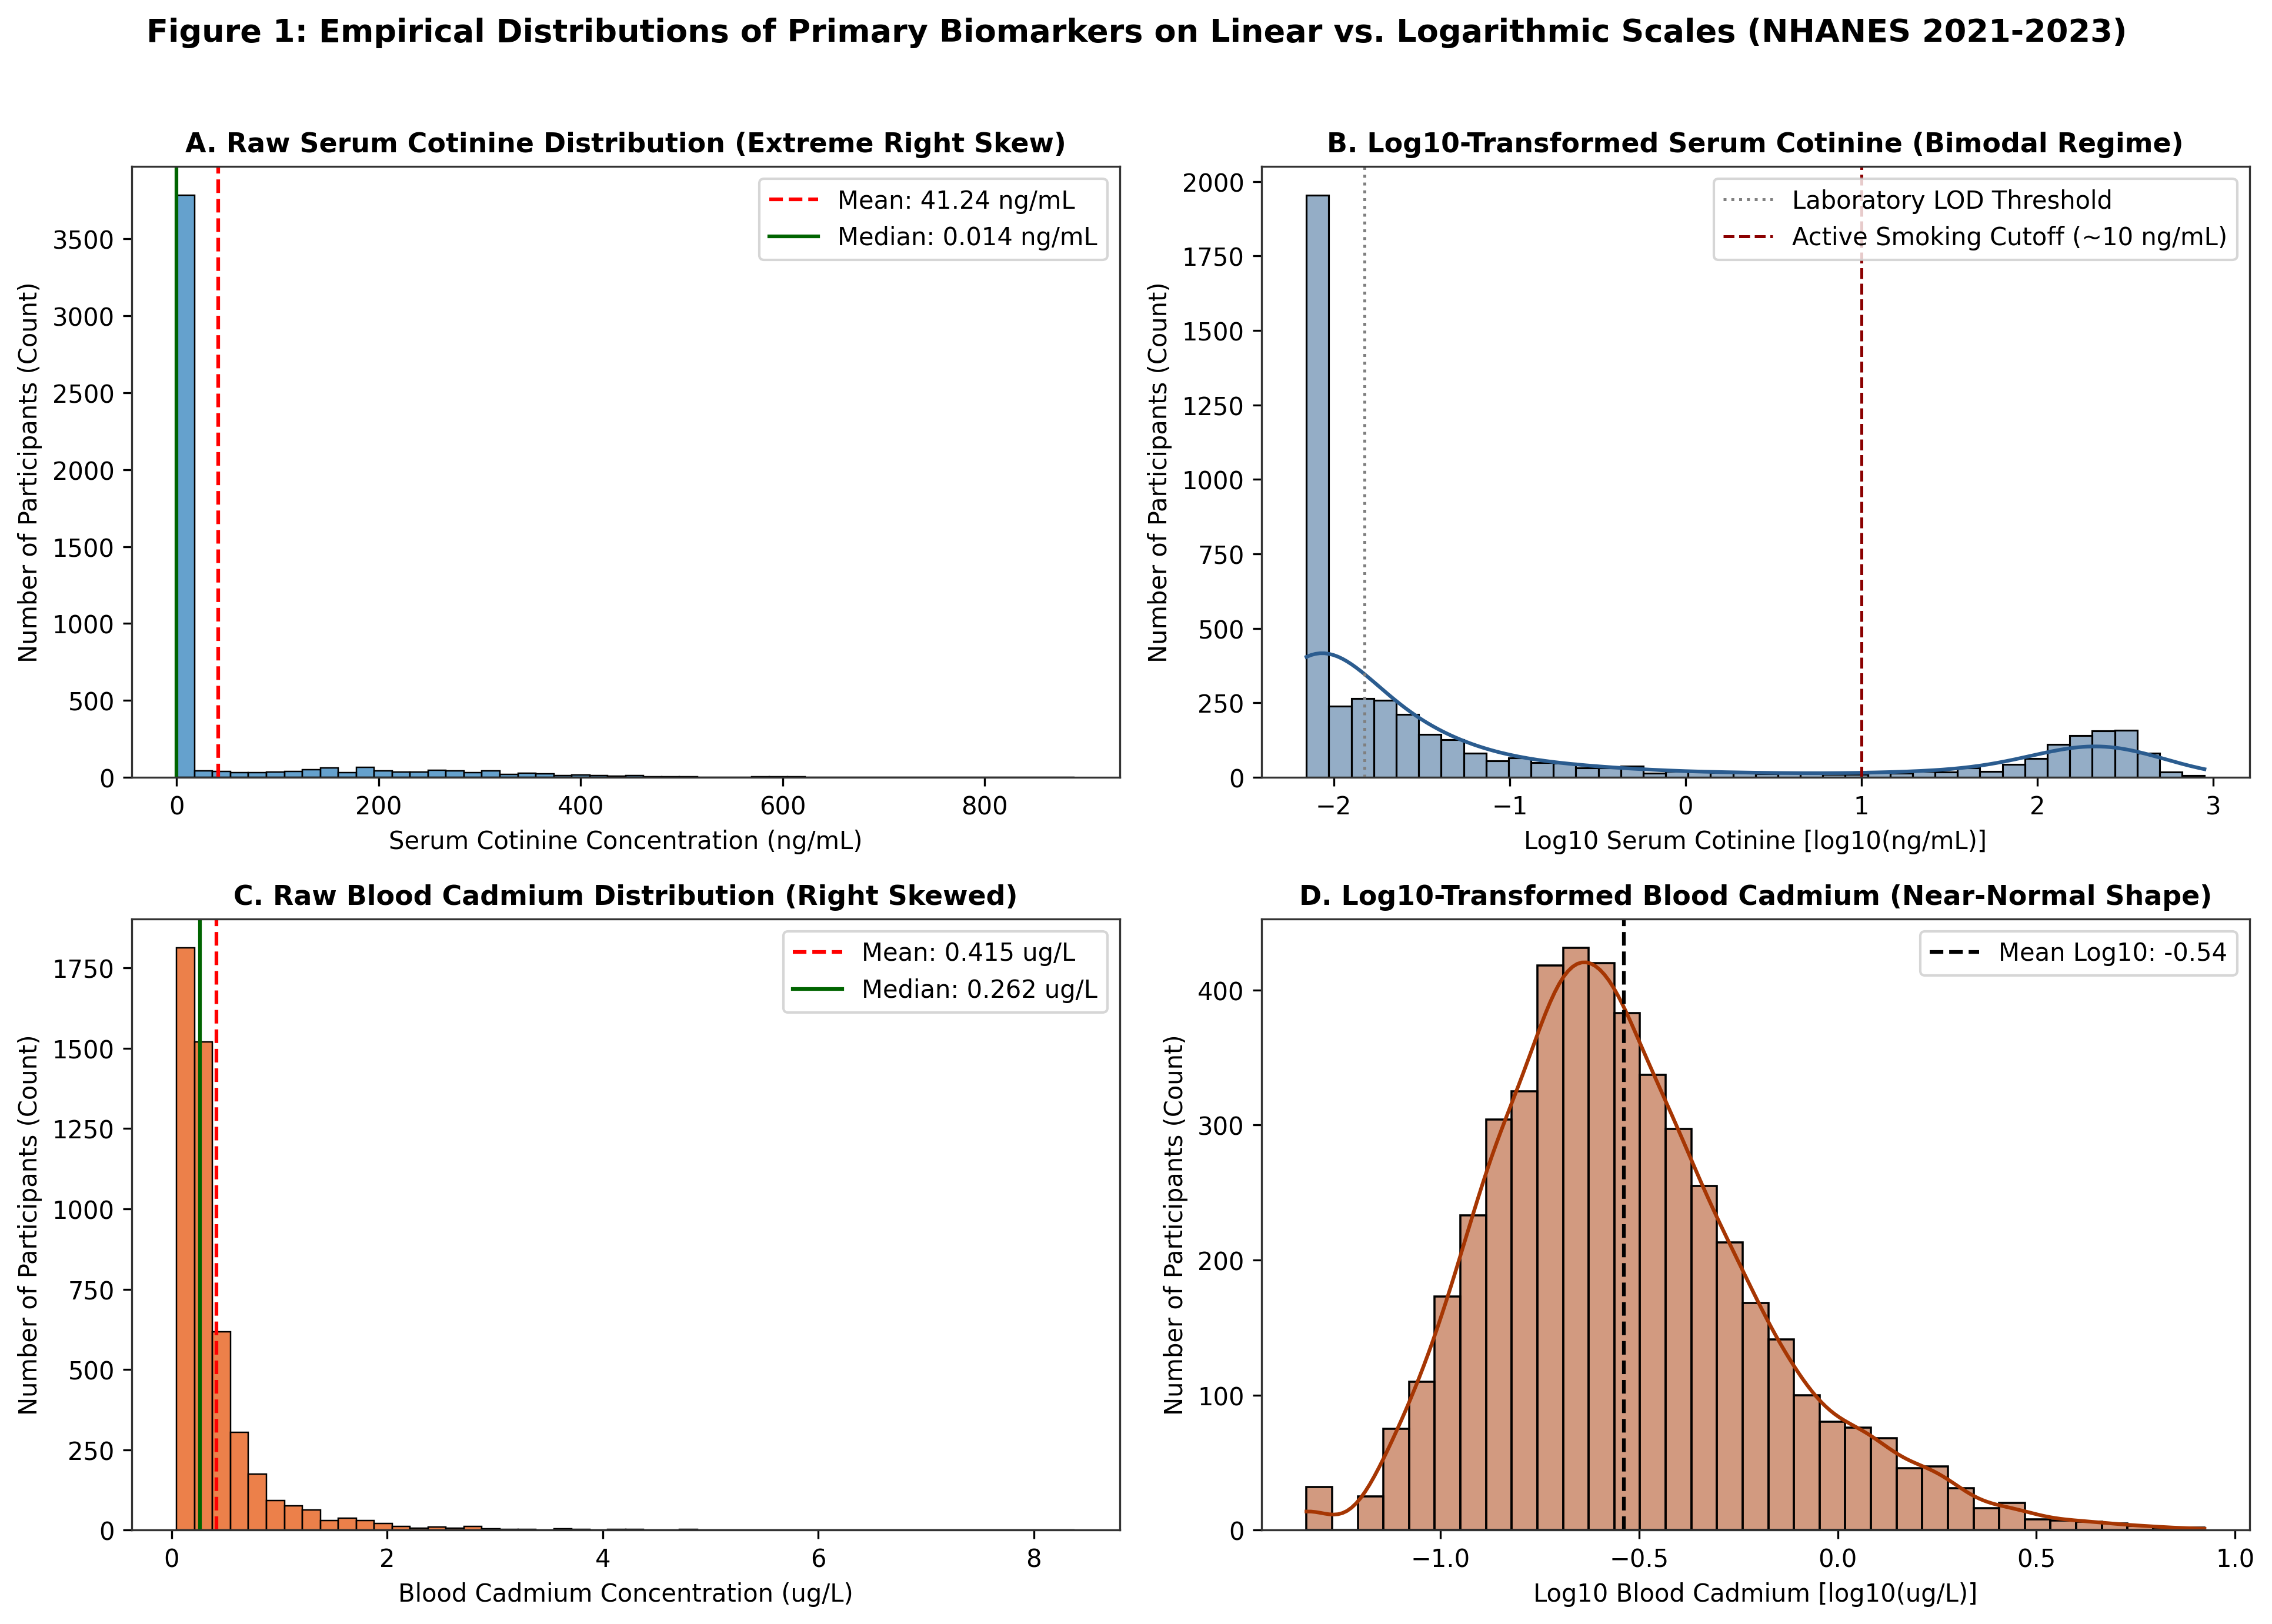
\includegraphics[width=0.80\textwidth]{figures/fig1_biomarker_distributions.png}
\caption{توزیع تجربی کوتینین سرم و کادمیوم خون در مقیاس خطی خام (چپ) و لگاریتمی پایه \lr{10} (راست).}
\end{figure}

\begin{figure}[htbp]
\centering
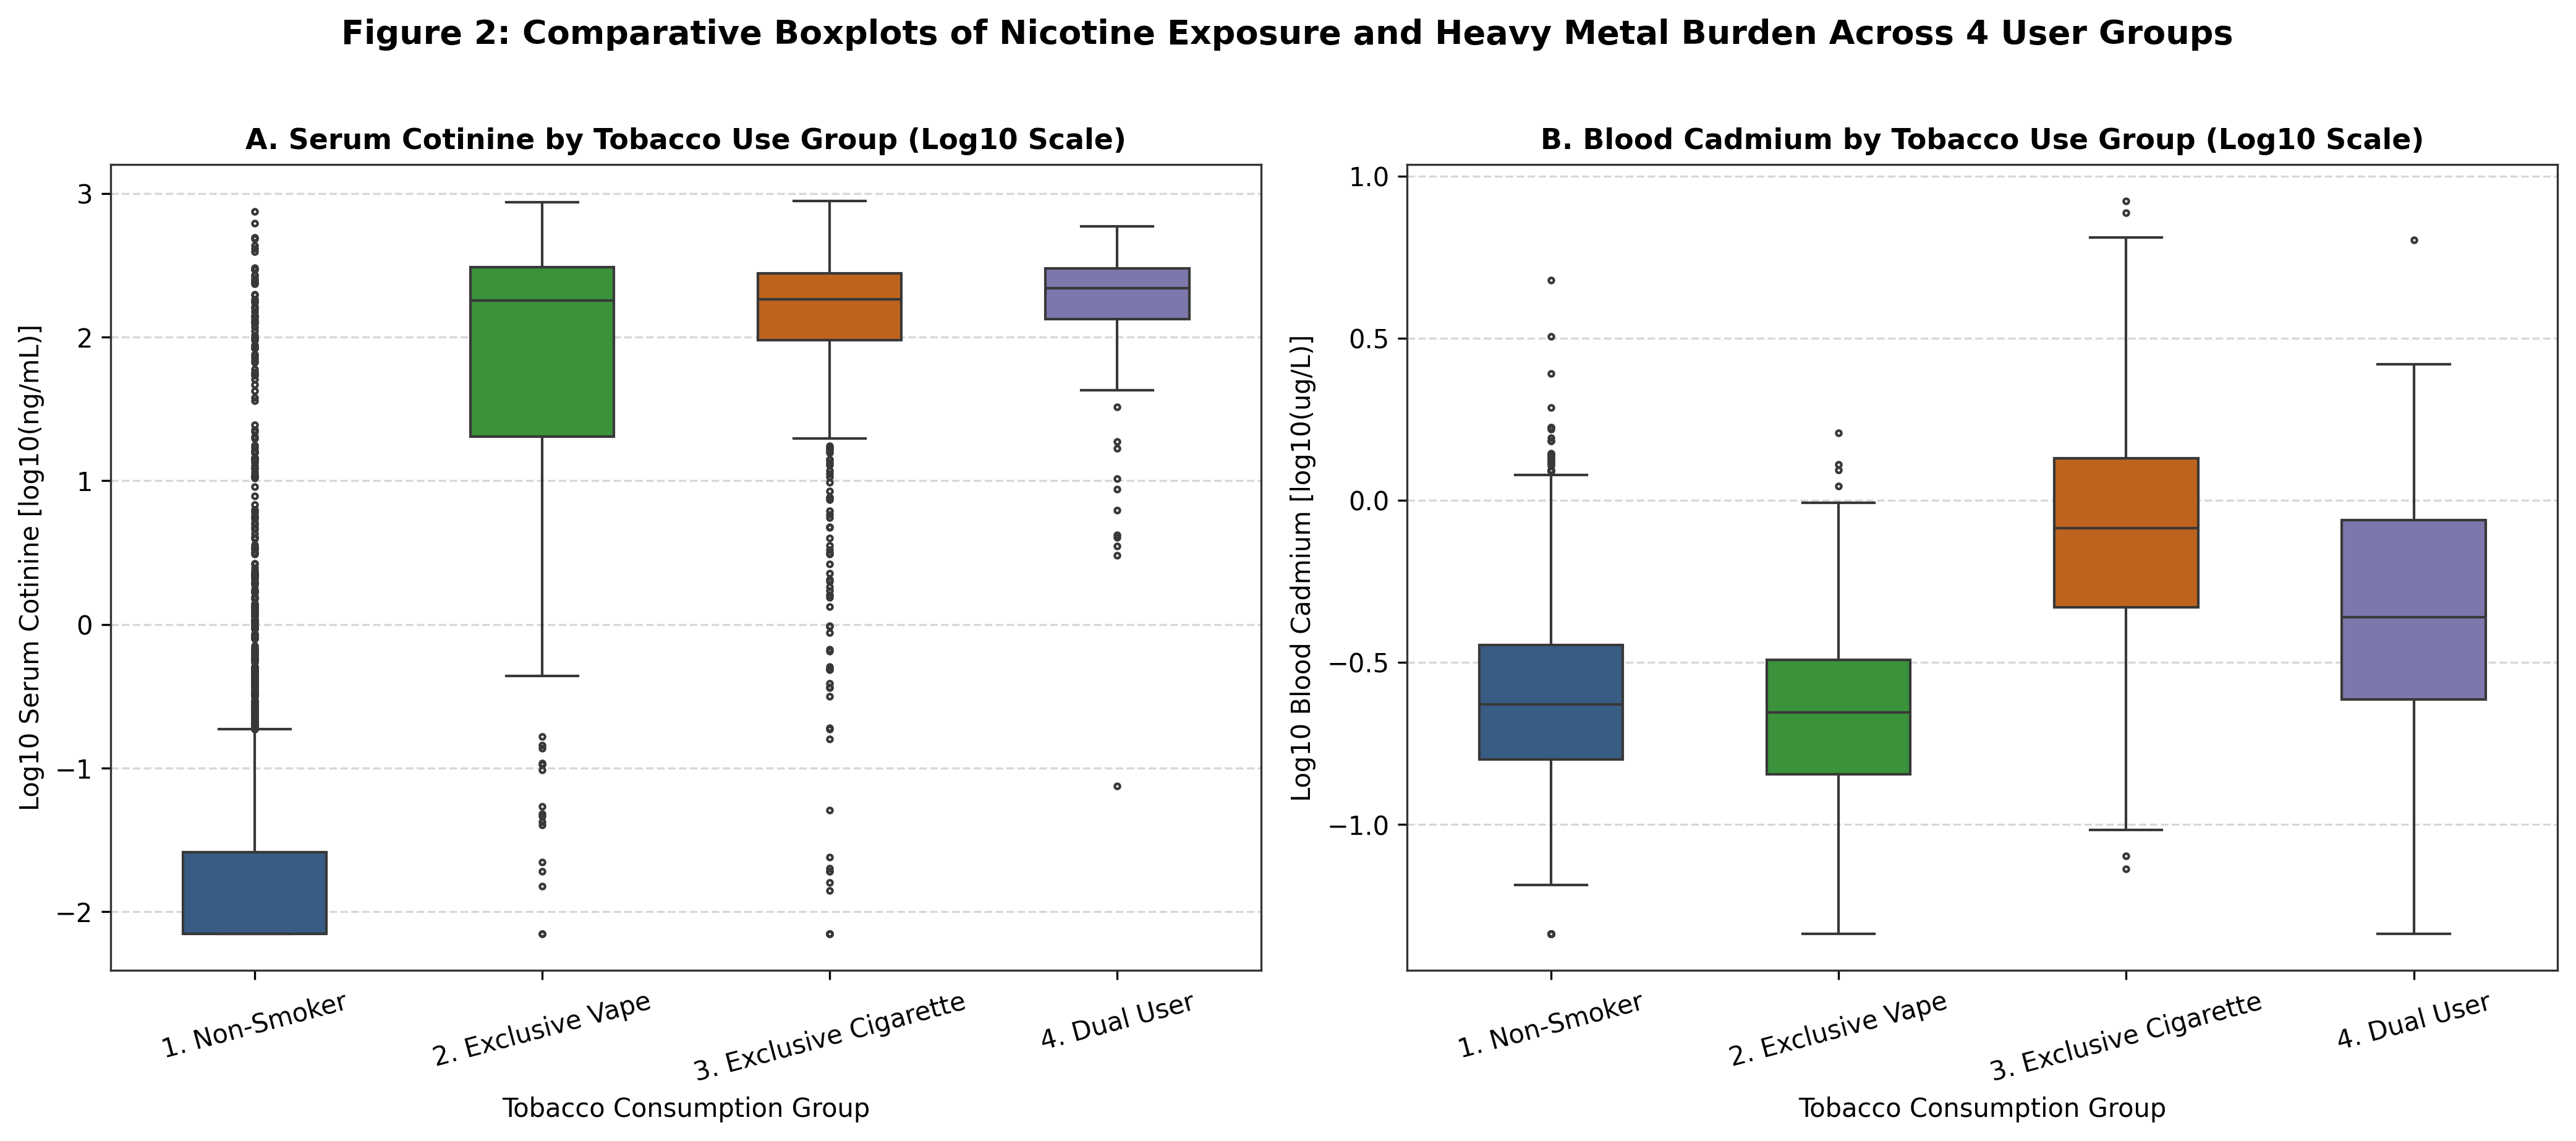
\includegraphics[width=0.80\textwidth]{figures/fig2_group_boxplots.png}
\caption{نمودار جعبه‌ای غلظت لگاریتمی کوتینین سرم (الف) و کادمیوم خون (ب) به تفکیک چهار گروه مصرف دخانیات.}
\end{figure}

\subsection{نمودار ۳ و ۴: ترکیب دموگرافیک گروه‌ها و رابطه دوز-پاسخ}
در شکل ۳ (پنل \lr{A})، سهم زنان در غیرسیگاری‌ها (\lr{57.4\%}) و ویپرها (\lr{53.0\%}) بیشتر است، اما در سیگاری‌های سنتی (\lr{53.9\%}) و مصرف دوگانه (\lr{57.3\%}) مردان اکثریت دارند. در پنل \lr{B} (نمودار انباشته \lr{100\%} تحصیلات)، سهم فارغ‌التحصیلان دانشگاه (بخش زرد) از حدود \lr{44\%} در غیرسیگاری‌ها و \lr{27\%} در ویپرها، به حدود \lr{12\%} تا \lr{15\%} در سیگاری‌های سنتی و دوگانه سقوط می‌کند. در شکل ۴ نیز رابطه دوز روزانه سیگار (\lr{SMQ720}) با کوتینین و کادمیوم، علاوه بر نمایش پدیده گرد کردن اعداد حول مضارب \lr{5} و \lr{10} نخ (\lr{Digit Preference})، یک شیب خطی کاملاً مثبت و صعودی را برای هر دو بیومارکر تایید می‌کند.

\begin{figure}[htbp]
\centering
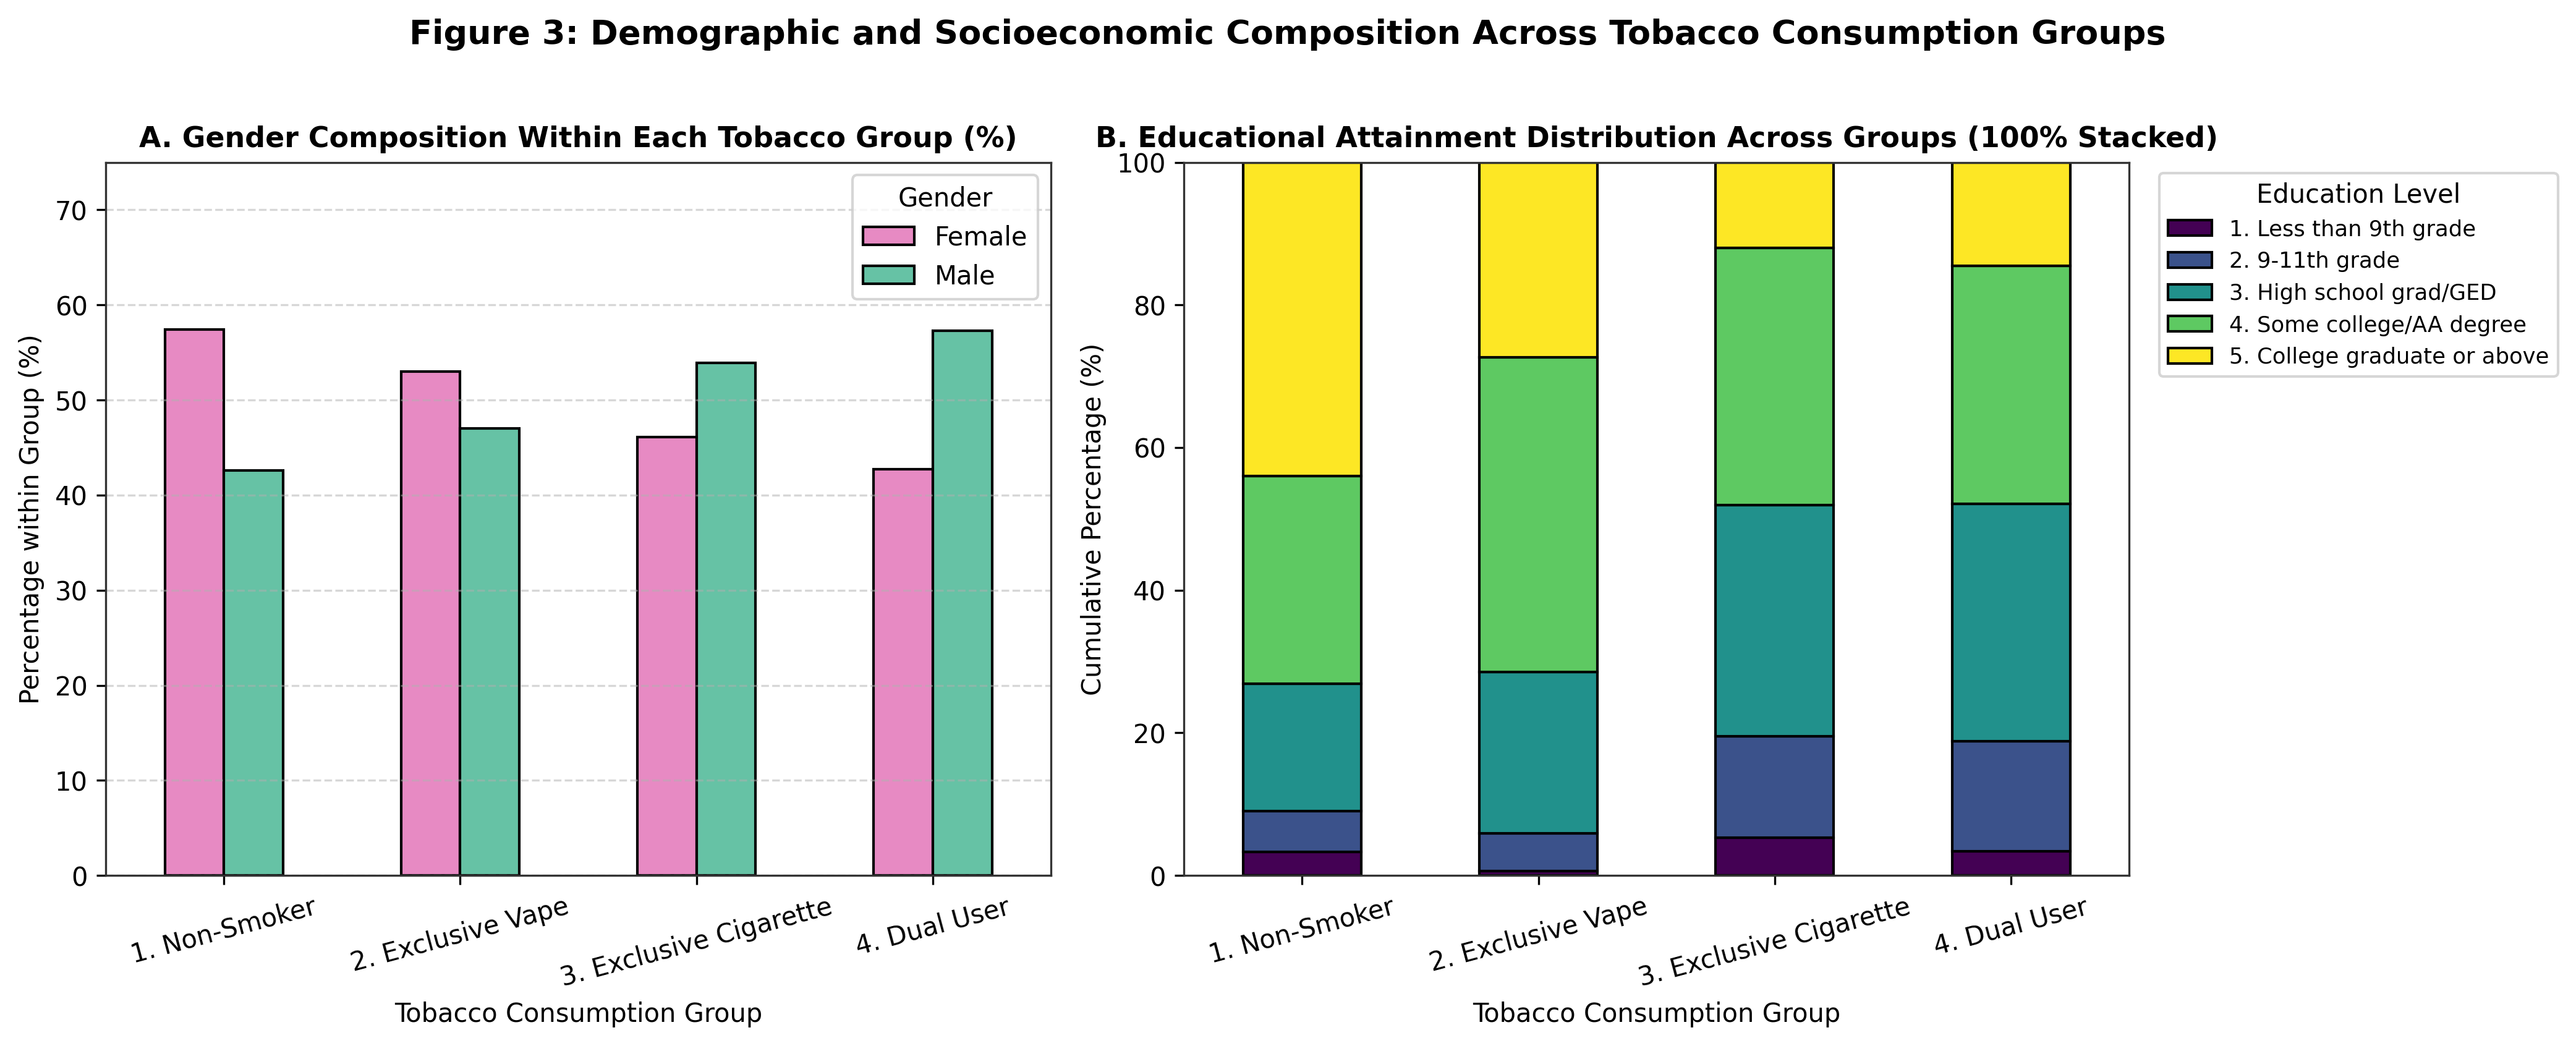
\includegraphics[width=0.80\textwidth]{figures/fig3_demographic_bars.png}
\caption{ترکیب جنسیتی (الف) و توزیع سطح تحصیلات (ب) در درون هر یک از چهار گروه مصرف دخانیات.}
\end{figure}

\begin{figure}[htbp]
\centering
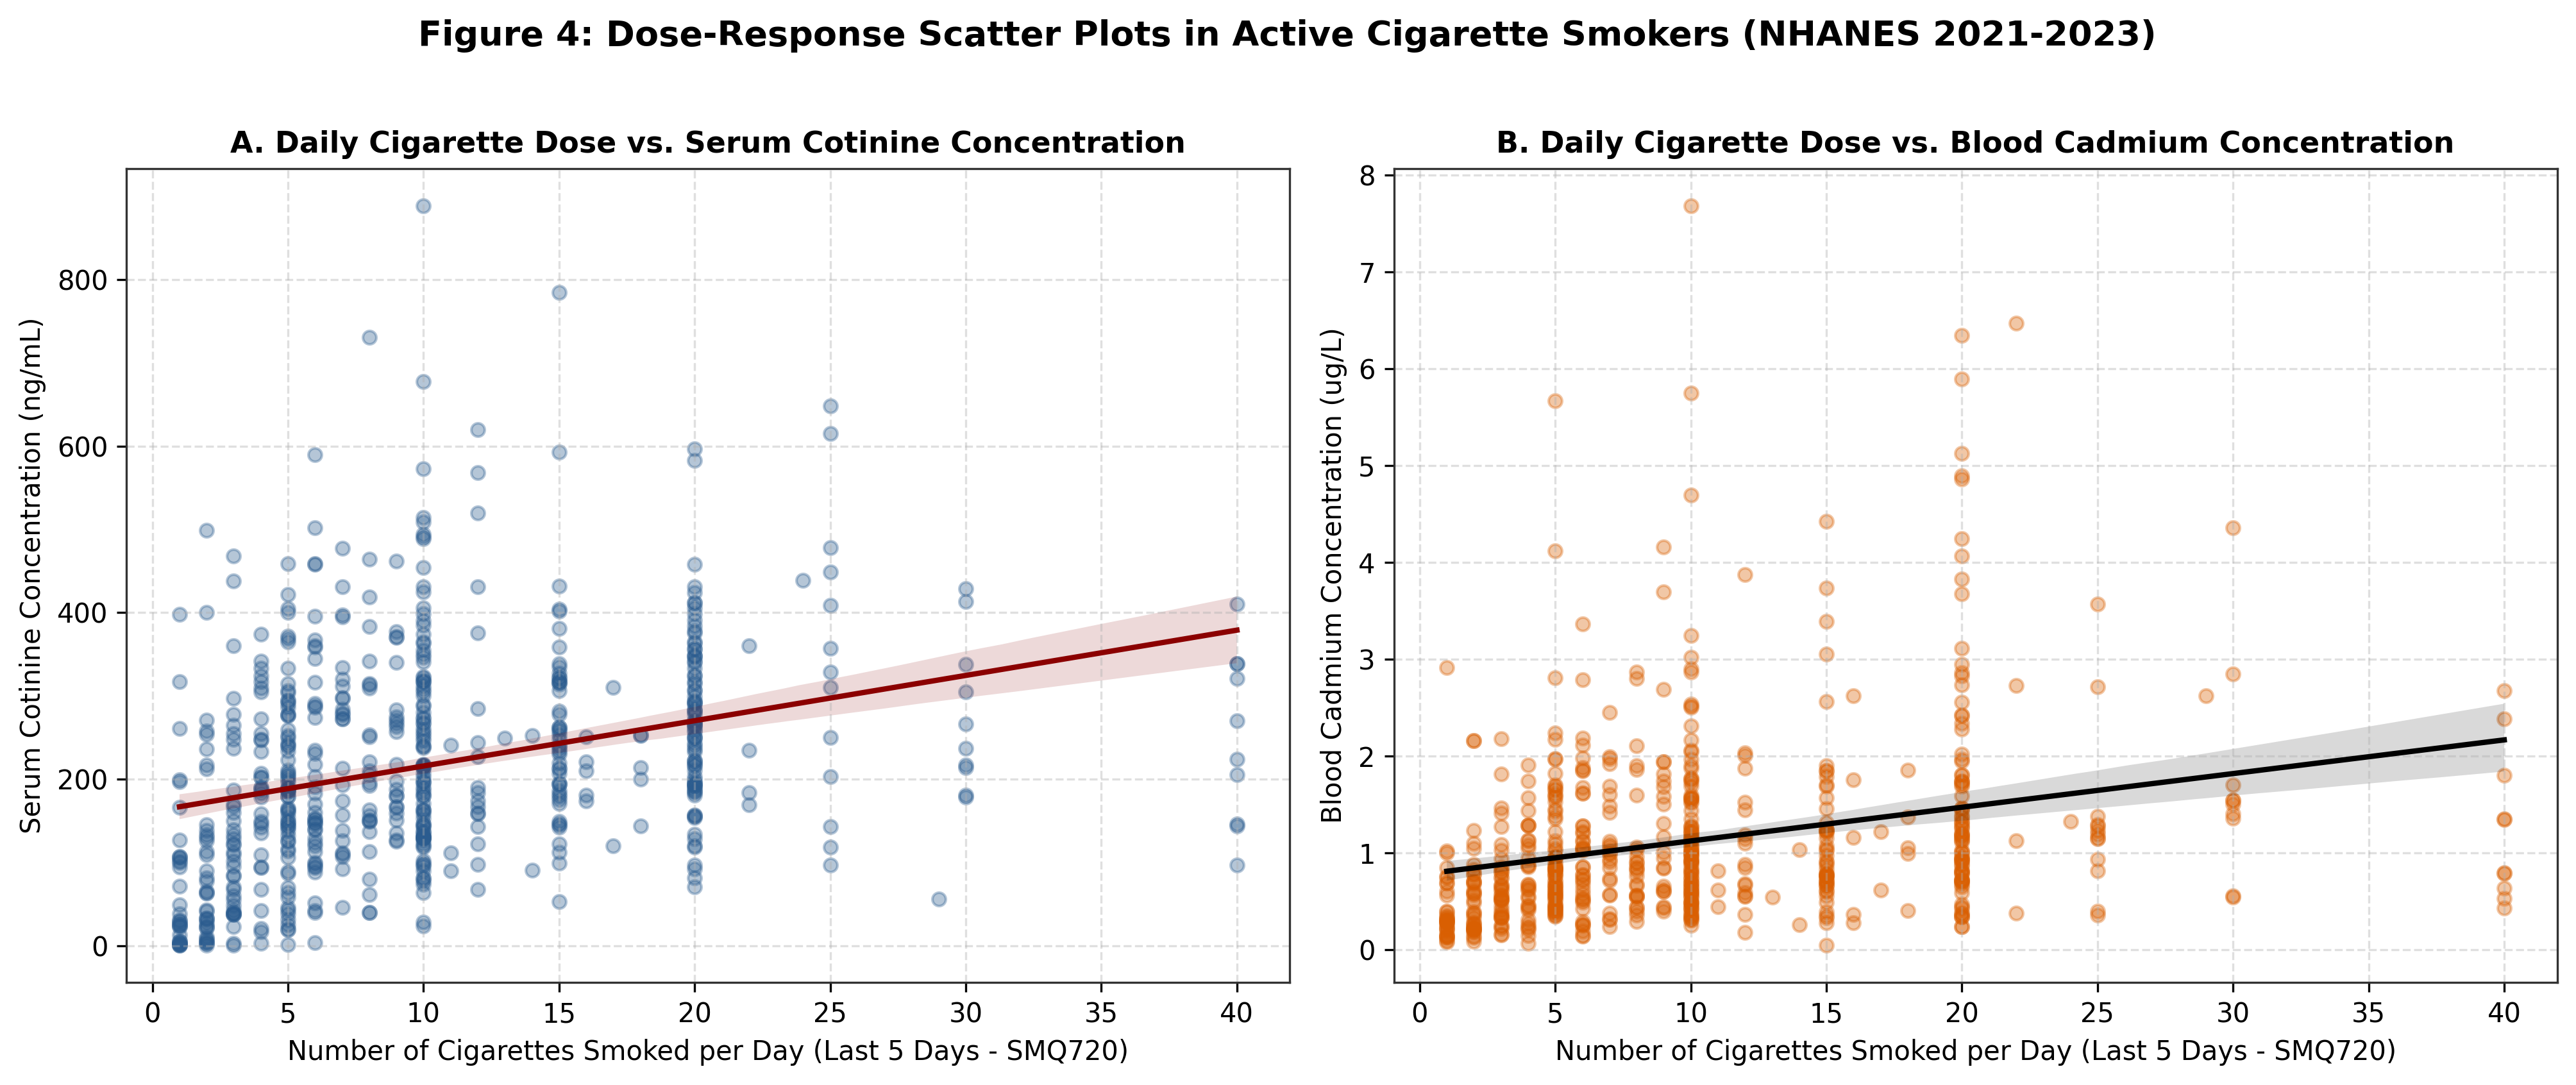
\includegraphics[width=0.80\textwidth]{figures/fig4_dose_response_scatter.png}
\caption{نمودار پراکنش و خط روند رابطه دوز مصرف روزانه سیگار با غلظت کوتینین سرم (الف) و کادمیوم خون (ب).}
\end{figure}


\section{مقایسه توصیفی اولیه میان گروه‌های مطالعه}

جدول زیر مقایسه توصیفی میانه (\lr{IQR}) و میانگین متغیرهای کمی را در چهار گروه مصرف دخانیات (بدون ادعای استنباطی) نشان می‌دهد:

\begin{table}[htbp]
\centering
\caption{مقایسه توصیفی میانه (\lr{IQR}) و میانگین متغیرهای کمی در چهار گروه مصرف دخانیات}
\resizebox{\textwidth}{!}{
\begin{tabular}{lllll}
\toprule
متغیر (واحد) & \lr{1. Non-Smoker} & \lr{2. Exclusive Vape} & \lr{3. Exclusive Cigarette} & \lr{4. Dual User} \\
 & میانه (\lr{IQR}) $\mid$ میانگین & میانه (\lr{IQR}) $\mid$ میانگین & میانه (\lr{IQR}) $\mid$ میانگین & میانه (\lr{IQR}) $\mid$ میانگین \\
\midrule
\lr{LBXCOT} (\lr{ng/mL}) & \lr{0.007} (\lr{0.019}) $\mid$ \lr{2.972} & \lr{180.500} (\lr{287.900}) $\mid$ \lr{187.476} & \lr{183.000} (\lr{182.700}) $\mid$ \lr{195.491} & \lr{219.000} (\lr{168.500}) $\mid$ \lr{215.231} \\
\lr{LBXHCOT} (\lr{ng/mL}) & \lr{0.003} (\lr{0.008}) $\mid$ \lr{1.525} & \lr{62.300} (\lr{126.810}) $\mid$ \lr{84.101} & \lr{75.750} (\lr{97.825}) $\mid$ \lr{93.781} & \lr{75.300} (\lr{94.500}) $\mid$ \lr{103.620} \\
\lr{LBXBCD} (\lr{ug/L}) & \lr{0.235} (\lr{0.199}) $\mid$ \lr{0.290} & \lr{0.222} (\lr{0.179}) $\mid$ \lr{0.280} & \lr{0.819} (\lr{0.880}) $\mid$ \lr{1.082} & \lr{0.436} (\lr{0.626}) $\mid$ \lr{0.710} \\
\lr{LBXBPB} (\lr{ug/dL}) & \lr{0.718} (\lr{0.636}) $\mid$ \lr{0.938} & \lr{0.623} (\lr{0.489}) $\mid$ \lr{0.746} & \lr{0.991} (\lr{0.805}) $\mid$ \lr{1.222} & \lr{0.735} (\lr{0.546}) $\mid$ \lr{1.132} \\
\lr{LBXBSE} (\lr{ug/L}) & \lr{178.100} (\lr{29.200}) $\mid$ \lr{181.862} & \lr{180.800} (\lr{23.775}) $\mid$ \lr{181.024} & \lr{176.400} (\lr{29.700}) $\mid$ \lr{177.445} & \lr{176.600} (\lr{29.150}) $\mid$ \lr{180.383} \\
\lr{LBXHGB} (\lr{g/dL}) & \lr{13.800} (\lr{1.800}) $\mid$ \lr{13.826} & \lr{14.000} (\lr{2.100}) $\mid$ \lr{14.033} & \lr{14.400} (\lr{2.000}) $\mid$ \lr{14.291} & \lr{14.600} (\lr{1.500}) $\mid$ \lr{14.420} \\
\lr{LBXWBCSI} (\lr{1000/uL})& \lr{6.500} (\lr{2.300}) $\mid$ \lr{6.727} & \lr{6.800} (\lr{3.000}) $\mid$ \lr{7.169} & \lr{7.500} (\lr{2.800}) $\mid$ \lr{7.667} & \lr{7.500} (\lr{2.800}) $\mid$ \lr{7.870} \\
\lr{RIDAGEYR} (سال) & \lr{59.000} (\lr{29.000}) $\mid$ \lr{55.191} & \lr{34.000} (\lr{25.250}) $\mid$ \lr{38.464} & \lr{56.000} (\lr{22.000}) $\mid$ \lr{53.165} & \lr{36.000} (\lr{25.000}) $\mid$ \lr{40.256} \\
\lr{INDFMPIR} (نسبت) & \lr{3.350} (\lr{3.215}) $\mid$ \lr{3.237} & \lr{2.850} (\lr{3.035}) $\mid$ \lr{2.911} & \lr{1.680} (\lr{2.080}) $\mid$ \lr{2.052} & \lr{1.955} (\lr{2.375}) $\mid$ \lr{2.291} \\
\bottomrule
\end{tabular}
}
\end{table}

\textbf{تحلیل یافته‌های توصیفی و شواهد مخدوش‌کنندگی (\lr{Confounding}):}
\begin{enumerate}
\item \textbf{جذب بالای نیکوتین در ویپرها و اوج مصرف در گروه دوگانه:} میانه کوتینین در انحصاری ویپ (\lr{180.500 ng/mL}) و انحصاری سیگار (\lr{183.000 ng/mL}) تقریباً برابر است و در مصرف دوگانه به اوج خود (\lr{219.000 ng/mL}) می‌رسد، در حالی که در غیرسیگاری‌ها \lr{0.007 ng/mL} است.
\item \textbf{واگرایی عظیم در کادمیوم (\lr{LBXBCD}) و سرب (\lr{LBXBPB}) و روند پلکانی التهاب (\lr{LBXWBCSI}):} میانه کادمیوم در سیگاری‌های سنتی (\lr{0.819 ug/L}) بیش از \lr{3.7} برابر مصرف‌کنندگان انحصاری ویپ (\lr{0.222 ug/L}) است و سطح کادمیوم ویپرها کاملاً منطبق بر غیرسیگاری‌ها (\lr{0.235 ug/L}) قرار دارد. همچنین شمارش گلبول سفید و هموگلوبین از غیرسیگاری (\lr{6.500} و \lr{13.800}) به سمت ویپ (\lr{6.800} و \lr{14.000}) و سیگار و دوگانه (\lr{7.500} و \lr{14.600}) افزایش پلکانی دارند.
\item \textbf{تبیین معمای کادمیوم با متغیر مخدوش‌کننده سن (فصل اول ووناکات):} چرا میانه کادمیوم و سرب در ویپرها حتی از غیرسیگاری‌ها اندکی کمتر است (\lr{0.222} در برابر \lr{0.235}) و در مصرف دوگانه کمتر از سیگار انحصاری است (\lr{0.436} در برابر \lr{0.819})؟ پاسخ در سطر سن (\lr{RIDAGEYR}) نهفته است: میانه سن ویپرها (\lr{34.0} سال) و دوگانه‌ها (\lr{36.0} سال) بیش از \lr{20} سال کمتر از غیرسیگاری‌ها (\lr{59.0} سال) و سیگاری‌های سنتی (\lr{56.0} سال) است! از آنجا که کادمیوم و سرب نیمه‌عمر تجمع \lr{10} تا \lr{30} ساله در بدن دارند، جوان بودن ویپرها سطح پایه فلزات سنگین آن‌ها را کاهش داده است. همچنین میانه نسبت درآمد به فقر در سیگاری‌ها (\lr{1.680}) بسیار کمتر از غیرسیگاری‌ها (\lr{3.350}) است. این یافته‌ها اثبات می‌کنند که کنترل هم‌زمان سن، درآمد و تحصیلات در رگرسیون فاز چهارم کاملاً حیاتی است.
\end{enumerate}


\section{نهایی‌سازی سؤال آماری پژوهش (تسک ۱۰)}

بر اساس شناخت تجربی حاصل از تسک‌های \lr{5} تا \lr{9}، سؤال آماری کارت پروژه در سه محور تدقیق شد: (۱) تغییر مقیاس متغیرهای پاسخ اصلی به مقیاس لگاریتمی (\lr{$\log_{10}$}) جهت رفع چولگی شدید، (۲) محدود کردن جامعه هدف به بزرگسالان \lr{20} سال و بالاترِ پالایش‌شده از تداخل قلیان، تنباکوی جویدنی و داروهای ترک نیکوتین در \lr{5} روز اخیر، و (۳) الزامی شدن کنترل آماری سن و طبقه اقتصادی-اجتماعی.

\textbf{صورت نهایی سؤال آماری:} «در جمعیت بزرگسالان غیرنظامی و غیرنهادی ایالات متحده (\lr{20} سال و بالاتر) در دوره پساکرونا (\lr{2021-2023})، پس از کنترل اثر متغیرهای مخدوش‌کننده سن (\lr{RIDAGEYR})، جنسیت (\lr{RIAGENDR})، تحصیلات (\lr{DMDEDUC2})، نسبت درآمد به فقر (\lr{INDFMPIR})، مواجهه با دود منزل (\lr{SMD470}) و سلنیوم خون (\lr{LBXBSE}) و با اعمال وزن خون‌گیری (\lr{WTPH2YR}): آیا مصرف‌کنندگان انحصاری ویپ در مقایسه با مصرف‌کنندگان سیگار سنتی و دوگانه، با وجود دریافت سطوح مشابه یا بالاتری از نیکوتین (\lr{LBXCOT} و \lr{LBXHCOT})، دارای بار تجمع کادمیوم و سرب خونی (\lr{LBXBCD} و \lr{LBXBPB}) و التهاب سیستمیک (\lr{LBXWBCSI}) به طور معنادار پایین‌تری هستند و آیا سطح فلزات سنگین خون آن‌ها با غیرسیگاری‌ها تفاوت معناداری دارد؟»

این مجموعه داده به دلیل دارا بودن سنجش‌های عینی آزمایشگاهی، پرسش‌نامه هم‌زمان \lr{5} روز اخیر در کلینیک، حجم نمونه کافی در هر چهار گروه (\lr{$n > 100$} در کوچک‌ترین گروه) و وزن اختصاصی \lr{WTPH2YR}، برای پاسخ به این سؤال کاملاً مناسب و کافی است.


\section{الزام الف-۱: شناسایی فایل‌ها، کلید ادغام و گزارش ابعاد}

در ماژول \lr{src/data\_loader.py}، هفت فایل خام با پایه قرار دادن فایل \lr{DEMO\_L} (\lr{11,933} نفر) از طریق کلید مشترک و یکتای فردی \lr{SEQN} به روش ادغام از چپ (\lr{Left Join}) به یکدیگر متصل شدند تا چارچوب کلی نمونه حفظ شود. همچنین اشتراک تجمعی (\lr{Cumulative Inner Join}) محاسبه گردید که نشان می‌دهد پس از اتصال پرسش‌نامه کلینیک (\lr{SMQRTU\_L})، اشتراک کامل روی \lr{7,199} نفر تثبیت می‌شود؛ زیرا تمامی پاسخ‌دهندگان به این پرسش‌نامه در فایل‌های آزمایشگاهی نیز حضور دارند:

\begin{table}[htbp]
\centering
\caption{ابعاد فایل‌های خام پیش از ادغام و گزارش گام‌به‌گام تعداد افراد قبل و بعد از هر مرحله ادغام روی کلید \lr{SEQN}}
\resizebox{\textwidth}{!}{
\begin{tabular}{llllllll}
\toprule
گام ادغام & نام فایل & شرح ماژول & کلید ادغام & سطرها (\lr{SEQN} یکتا) & ستون کل (منتخب) & سطرهای \lr{Left Join} & اشتراک تجمعی (\lr{Inner}) \\
\midrule
گام ۱ (پایه) & \lr{DEMO\_L} & جمعیت‌شناختی و وزن پایه & \lr{SEQN} & \lr{11,933} (\lr{11,933}) & \lr{27} (\lr{10}) & \lr{11,933} & \lr{11,933} \\
گام ۲ & \lr{SMQ\_L} & تاریخچه سیگار (\lr{12+} سال) & \lr{SEQN} & \lr{9,015} (\lr{9,015}) & \lr{9} (\lr{4}) & \lr{11,933} & \lr{9,015} \\
گام ۳ & \lr{SMQRTU\_L} & مصرف \lr{5} روز اخیر در \lr{MEC} & \lr{SEQN} & \lr{7,199} (\lr{7,199}) & \lr{21} (\lr{9}) & \lr{11,933} & \lr{7,199} \\
گام ۴ & \lr{SMQFAM\_L} & افراد سیگاری داخل منزل & \lr{SEQN} & \lr{11,933} (\lr{11,933}) & \lr{3} (\lr{2}) & \lr{11,933} & \lr{7,199} \\
گام ۵ & \lr{COT\_L} & کوتینین سرم (\lr{3+} سال) & \lr{SEQN} & \lr{8,493} (\lr{8,493}) & \lr{5} (\lr{5}) & \lr{11,933} & \lr{7,199} \\
گام ۶ & \lr{PBCD\_L} & فلزات سنگین خون (\lr{1+} سال) & \lr{SEQN} & \lr{8,727} (\lr{8,727}) & \lr{17} (\lr{8}) & \lr{11,933} & \lr{7,199} \\
گام ۷ & \lr{CBC\_L} & شمارش سلول‌های خونی (\lr{1+} سال) & \lr{SEQN} & \lr{8,727} (\lr{8,727}) & \lr{23} (\lr{3}) & \lr{11,933} & \lr{7,199} \\
\bottomrule
\end{tabular}
}
\end{table}


\section{الزام الف-۲: شناسایی وزن و طرح نمونه‌گیری}

برخلاف نمونه‌گیری تصادفی ساده که در آن شانس انتخاب هر فرد یکسان ($\pi_i = \frac{n}{N}$) است، در طرح چهارمرحله‌ای \lr{NHANES} هر فرد نماینده تعداد متفاوتی از افراد جمعیت ایالات متحده است ($w_i \neq w_j$). این تفاوت وزن ناشی از سه عامل است: (۱) معکوس احتمال نابرابر انتخاب ($w_{i,\text{base}} = \frac{1}{\pi_i}$)، به طوری که بزرگسالان \lr{20} تا \lr{59} ساله به دلیل انتخاب تصادفی در خانوار، وزن پایه بزرگ‌تری نسبت به سالمندان \lr{60+} سال (که \lr{100\%} انتخاب شده‌اند) دریافت می‌کنند؛ (۲) ضرب شدن در ضریب تعدیل عدم پاسخ در زیرگروه‌ها؛ و (۳) کالیبراسیون نهایی (\lr{Raking}) با آمار سرشماری رسمی آمریکا.

بر اساس «اصل کوچک‌ترین زیرجمعیت» (\lr{Smallest Subpopulation Principle})، از میان سه وزن موجود (\lr{WTINT2YR}، \lr{WTMEC2YR} و \lr{WTPH2YR})، متغیر \lr{\textbf{WTPH2YR}} (وزن دو ساله خون‌گیری) تنها وزن صحیح برای این پژوهش است. جدول زیر نشان می‌دهد که با وجود کاهش تعداد بزرگسالان از مصاحبه (\lr{7,809} نفر) به خون‌گیری (\lr{5,792} نفر)، مجموع وزن‌ها در هر سه متغیر دقیقاً برابر با \lr{245,061,169} نفر (کل جمعیت بزرگسال غیرنظامی آمریکا) ثابت مانده است و در \lr{WTPH2YR} هر فرد نماینده \lr{4,391.8} تا \lr{241,728.9} نفر (نسبت \lr{55.0} برابر) است:

\begin{table}[htbp]
\centering
\caption{مشخصات و دامنه تغییرات وزن‌های نمونه‌گیری در زیرجمعیت بزرگسالان (\lr{20} سال و بالاتر)}
\resizebox{\textwidth}{!}{
\begin{tabular}{llllllll}
\toprule
متغیر وزن & تعداد وزن مثبت & مجموع وزن‌ها (جمعیت بزرگسال آمریکا) & کمینه وزن & میانه وزن & میانگین وزن & بیشینه وزن & نسبت بیشینه به کمینه \\
\midrule
\lr{WTINT2YR} & \lr{7,809} & \lr{245,061,169} & \lr{4,584.5} & \lr{25,135.1} & \lr{31,381.9} & \lr{170,968.3} & \lr{37.3} \\
\lr{WTMEC2YR} & \lr{6,064} & \lr{245,061,169} & \lr{4,581.6} & \lr{31,816.9} & \lr{40,412.5} & \lr{227,108.3} & \lr{49.6} \\
\lr{WTPH2YR} & \lr{5,792} & \lr{245,061,169} & \lr{4,391.8} & \lr{33,332.9} & \lr{42,310.3} & \lr{241,728.9} & \lr{55.0} \\
\bottomrule
\end{tabular}
}
\end{table}


\section{الزام الف-۳: مقایسه خلاصه‌های خام و وزن‌دار}

در این بخش، مطابق با فرمول میانگین موزون در فصل دوم کتاب ووناکات ($\bar{X}_w = \frac{\sum w_i X_i}{\sum w_i}$)، شاخص‌های کمی و نسبت‌های طبقه‌ای در جمعیت تحلیلی نهایی (\lr{$N = 4,655$}) در دو حالت بدون وزن (\lr{Unweighted}) و وزن‌دار (\lr{Weighted} با \lr{WTPH2YR}) مقایسه شده‌اند:

\begin{table}[htbp]
\centering
\caption{مقایسه میانگین و میانه خام (\lr{Unweighted}) و وزن‌دار (\lr{WTPH2YR}) برای متغیرهای کمی در جمعیت تحلیلی}
\resizebox{\textwidth}{!}{
\begin{tabular}{llllllll}
\toprule
متغیر و شرح & تعداد (\lr{$n$}) & میانگین خام & میانگین وزن‌دار & اختلاف میانگین & تغییر نسبی (\lr{\%}) & میانه خام & میانه وزن‌دار \\
\midrule
\lr{RIDAGEYR} (سن کل نمونه تحلیلی) & \lr{4,655} & \lr{54.133} & \lr{48.997} & \lr{-5.136} & \lr{-9.49\%} & \lr{58.000} & \lr{49.000} \\
\lr{INDFMPIR} (نسبت درآمد به فقر) & \lr{4,103} & \lr{3.071} & \lr{3.139} & \lr{+0.067} & \lr{+2.20\%} & \lr{3.080} & \lr{3.220} \\
\lr{LBXCOT} (کوتینین سرم - کل) & \lr{4,655} & \lr{41.248} & \lr{41.714} & \lr{+0.465} & \lr{+1.13\%} & \lr{0.014} & \lr{0.016} \\
\lr{LBXBCD} (کادمیوم خون - کل) & \lr{4,655} & \lr{0.408} & \lr{0.378} & \lr{-0.030} & \lr{-7.24\%} & \lr{0.262} & \lr{0.238} \\
\lr{LBXBPB} (سرب خون - کل) & \lr{4,655} & \lr{0.973} & \lr{0.891} & \lr{-0.082} & \lr{-8.41\%} & \lr{0.742} & \lr{0.672} \\
\lr{LBXHGB} (هموگلوبین خون) & \lr{4,638} & \lr{13.909} & \lr{14.000} & \lr{+0.091} & \lr{+0.65\%} & \lr{13.900} & \lr{14.100} \\
\lr{LBXWBCSI} (گلبول سفید خون) & \lr{4,638} & \lr{6.890} & \lr{6.899} & \lr{+0.009} & \lr{+0.13\%} & \lr{6.600} & \lr{6.600} \\
\midrule
\lr{LBXCOT} در گروه \lr{2. Exclusive Vape} & \lr{146} & \lr{187.476} & \lr{201.020} & \lr{+13.544} & \lr{+7.22\%} & \lr{180.500} & \lr{191.000} \\
\lr{LBXBCD} در گروه \lr{2. Exclusive Vape} & \lr{146} & \lr{0.274} & \lr{0.236} & \lr{-0.038} & \lr{-13.76\%} & \lr{0.218} & \lr{0.183} \\
\lr{LBXCOT} در گروه \lr{3. Exclusive Cigarette} & \lr{672} & \lr{195.491} & \lr{182.137} & \lr{-13.354} & \lr{-6.83\%} & \lr{183.000} & \lr{175.000} \\
\lr{LBXBCD} در گروه \lr{3. Exclusive Cigarette} & \lr{672} & \lr{1.059} & \lr{1.011} & \lr{-0.048} & \lr{-4.54\%} & \lr{0.794} & \lr{0.764} \\
\lr{LBXCOT} در گروه \lr{4. Dual User} & \lr{103} & \lr{215.231} & \lr{218.321} & \lr{+3.091} & \lr{+1.44\%} & \lr{219.000} & \lr{227.000} \\
\lr{LBXBCD} در گروه \lr{4. Dual User} & \lr{103} & \lr{0.694} & \lr{0.604} & \lr{-0.090} & \lr{-12.96\%} & \lr{0.432} & \lr{0.378} \\
\bottomrule
\end{tabular}
}
\end{table}

\begin{table}[htbp]
\centering
\caption{مقایسه نسبت‌ها (درصدهای) خام و وزن‌دار (\lr{WTPH2YR}) برای متغیرهای طبقه‌ای در جمعیت تحلیلی (\lr{$N = 4,655$})}
\resizebox{0.92\textwidth}{!}{
\begin{tabular}{llllll}
\toprule
متغیر طبقه‌ای & طبقه / زیرگروه & تعداد در نمونه (\lr{$n$}) & درصد خام (\lr{\%}) & درصد وزن‌دار (\lr{\%}) & اختلاف (\lr{W - Unw}) \\
\midrule
گروه مصرف دخانیات & \lr{1. Non-Smoker} (غیرسیگاری) & \lr{3,734} & \lr{80.21\%} & \lr{79.42\%} & \lr{-0.80\%} \\
 & \lr{2. Exclusive Vape} (انحصاری ویپ) & \lr{146} & \lr{3.14\%} & \lr{3.86\%} & \lr{+0.73\%} \\
 & \lr{3. Exclusive Cigarette} (انحصاری سیگار) & \lr{672} & \lr{14.44\%} & \lr{13.99\%} & \lr{-0.44\%} \\
 & \lr{4. Dual User} (مصرف دوگانه) & \lr{103} & \lr{2.21\%} & \lr{2.73\%} & \lr{+0.52\%} \\
\midrule
گروه سنی & سالمندان (\lr{60} سال و بالاتر) & \lr{2,178} & \lr{46.79\%} & \lr{31.82\%} & \lr{-14.97\%} \\
\midrule
نژاد و قومیت & سفیدپوست غیرهیسپانیک / سیاه‌پوست & \lr{2,896} / \lr{499} & \lr{62.21\%} / \lr{10.72\%} & \lr{62.62\%} / \lr{10.49\%} & \lr{+0.40\%} / \lr{-0.23\%} \\
\bottomrule
\end{tabular}
}
\end{table}

\textbf{تحلیل اثر وزن‌دهی:} (۱) به دلیل انتخاب \lr{100\%} سالمندان در طراحی نمونه، افراد \lr{60+} سال در نمونه خام \lr{46.79\%} بودند؛ با اعمال وزن \lr{WTPH2YR}، سهم آن‌ها \lr{14.97\%} کاهش یافته و به نسبت واقعی جامعه (\lr{31.82\%}) بازمی‌گردد. در نتیجه، میانگین سن از \lr{54.133} به \lr{48.997} سال (\lr{-5.136} سال) و میانه سن از \lr{58.0} به \lr{49.0} سال کاهش می‌یابد و به تبع آن، میانگین کل کادمیوم (\lr{-7.24\%}) و سرب خون (\lr{-8.41\%}) در جامعه کم می‌شود. (۲) با افزایش وزن جوانان، شیوع انحصاری ویپ از \lr{3.14\%} به \lr{3.86\%} و مصرف دوگانه از \lr{2.21\%} به \lr{2.73\%} افزایش می‌یابد. (۳) در مقایسه درون‌گروهی وزن‌دار، میانگین کوتینین ویپرها به \lr{201.020 ng/mL} (میانه \lr{191.000}) می‌رسد که حتی از سیگاری‌های سنتی (\lr{182.137 ng/mL}) بالاتر است، در حالی که میانگین وزن‌دار کادمیوم در سیگاری‌ها (\lr{1.011 ug/L}) بیش از \lr{4.2} برابر ویپرها (\lr{0.236 ug/L}) باقی می‌ماند.


\section{الزام الف-۴: تعریف دقیق جمعیت تحلیلی و گزارش ریزش نمونه}

در ماژول \lr{src/survey\_design.py}، پنج معیار ورود و خروج متوالی بر روی دیتافریم اولیه (\lr{11,933} نفر) اعمال شد: (۱) ورود بزرگسالان \lr{20} سال و بالاتر (حذف \lr{4,124} کودک و نوجوان زیر \lr{20} سال)، (۲) داشتن وزن خون‌گیری مثبت \lr{$\text{WTPH2YR} > 0$} (حذف \lr{2,017} نفر)، (۳) کامل بودن هر دو پیامد اصلی کوتینین \lr{LBXCOT} و کادمیوم \lr{LBXBCD} (حذف \lr{272} نفر)، (۴) حذف مصرف‌کنندگان داروهای ترک نیکوتین (\lr{SMQ863=1})، قلیان (\lr{SMQ845=1}) و تنباکوی جویدنی (\lr{SMQ851=1}) در \lr{5} روز اخیر جهت رفع تداخل بیولوژیکی (حذف \lr{152} نفر)، و (۵) داشتن اطلاعات کامل پرسش‌نامه دخانیات برای تخصیص قطعی به یکی از \lr{4} گروه (حذف \lr{713} نفر).

\begin{table}[htbp]
\centering
\caption{جریان تعریف جمعیت تحلیلی و تعداد دقیق افراد حذف‌شده در هر مرحله}
\resizebox{\textwidth}{!}{
\begin{tabular}{llllll}
\toprule
گام & شرح معیار ورود / خروج اعمال‌شده & افراد باقی‌مانده & حذف‌شده در گام & حذف تجمعی & درصد ماندگاری \\
\midrule
گام ۰ & کل شرکت‌کنندگان در فایل ادغام‌شده اولیه (\lr{DEMO\_L}) & \lr{11,933} & \lr{0} & \lr{0} & \lr{100.00\%} \\
گام ۱ & محدودیت سنی: بزرگسالان \lr{20} سال و بالاتر (\lr{$\text{RIDAGEYR} \ge 20$}) & \lr{7,809} & \lr{4,124} & \lr{4,124} & \lr{65.44\%} \\
گام ۲ & داشتن وزن خون‌گیری مثبت و معتبر (\lr{$\text{WTPH2YR} > 0$}) & \lr{5,792} & \lr{2,017} & \lr{6,141} & \lr{48.54\%} \\
گام ۳ & موجود بودن هر دو پیامد اصلی کوتینین (\lr{LBXCOT}) و کادمیوم (\lr{LBXBCD}) & \lr{5,520} & \lr{272} & \lr{6,413} & \lr{46.26\%} \\
گام ۴ & حذف مصرف‌کنندگان داروهای ترک نیکوتین، قلیان و تنباکوی جویدنی & \lr{5,368} & \lr{152} & \lr{6,565} & \lr{44.98\%} \\
گام ۵ & اطلاعات کامل جهت طبقه‌بندی در یکی از \lr{4} گروه (جمعیت تحلیلی نهایی) & \lr{4,655} & \lr{713} & \lr{7,278} & \lr{39.01\%} \\
\bottomrule
\end{tabular}
}
\end{table}

در نهایت، جمعیت تحلیلی نهایی شامل \lr{\textbf{4,655}} بزرگسال واجد شرایط است که در چهار گروه مطالعه به صورت \lr{\textbf{3,734}} نفر غیرسیگاری (\lr{80.21\%} خام $\mid$ \lr{79.42\%} وزن‌دار)، \lr{\textbf{146}} نفر مصرف‌کننده انحصاری ویپ (\lr{3.14\%} خام $\mid$ \lr{3.86\%} وزن‌دار)، \lr{\textbf{672}} نفر مصرف‌کننده انحصاری سیگار سنتی (\lr{14.44\%} خام $\mid$ \lr{13.99\%} وزن‌دار) و \lr{\textbf{103}} نفر مصرف‌کننده دوگانه (\lr{2.21\%} خام $\mid$ \lr{2.73\%} وزن‌دار) توزیع شده‌اند و مبنای استنباط‌های فازهای بعدی را تشکیل می‌دهند.

\end{document}
